% !TEX root = ../PhD Thesis.tex

%\chapter{cTRAP: identification of candidate causal perturbations from differential gene expression data}
\chapter{cTRAP}
\label{chap:ctrap}

\begin{figure}[!b]
  \vspace*{-1cm}
  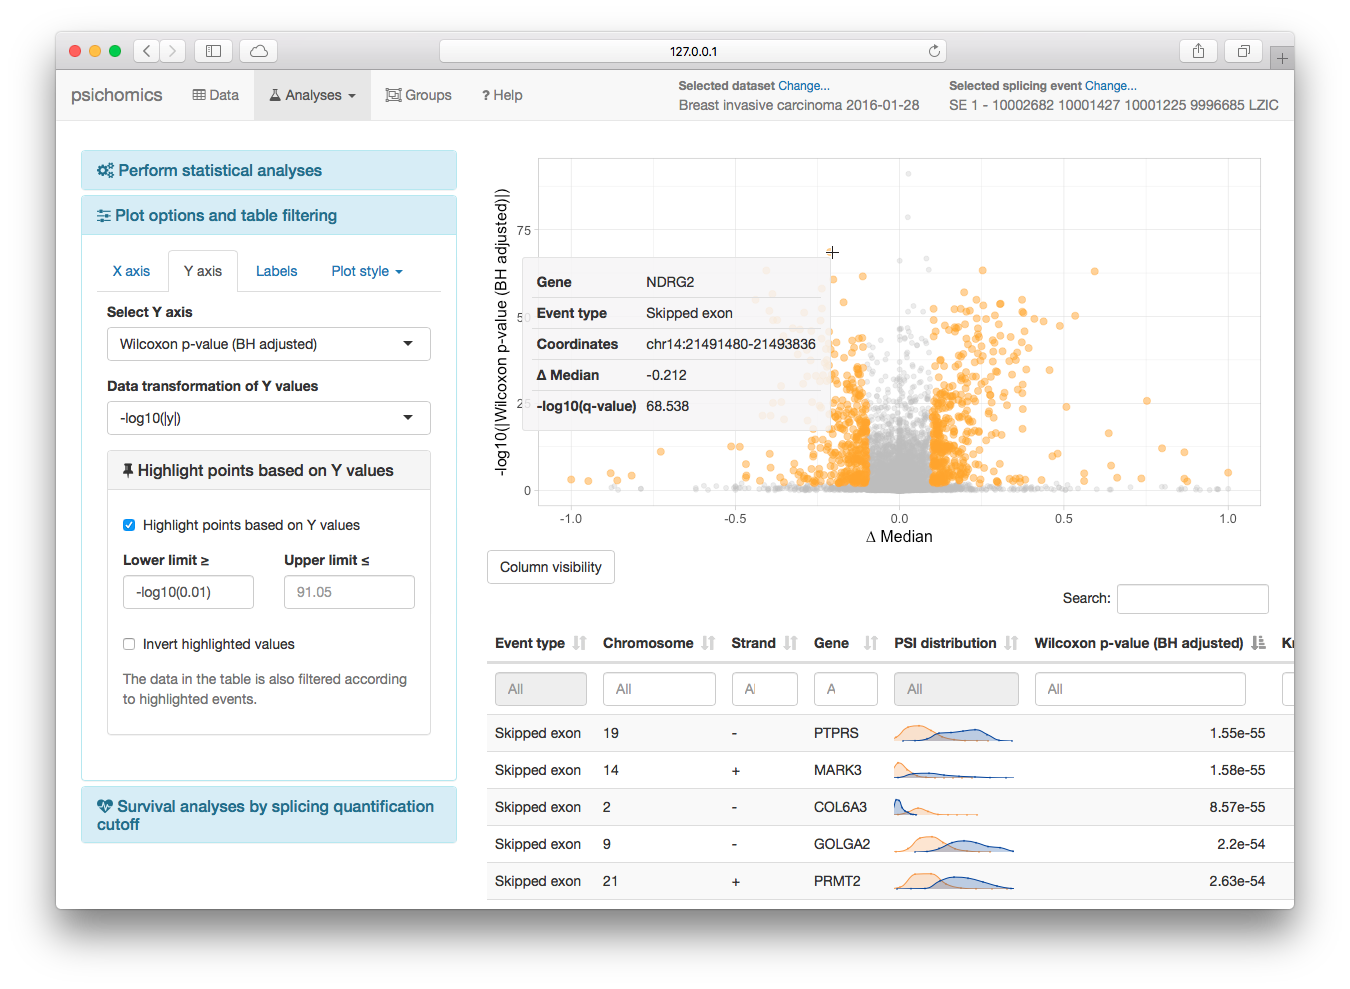
\includegraphics[width=.96\textwidth]{images/cTRAP/screenshot}
  \centering
  \vspace*{-.5cm}
  \caption[cTRAP global interface screenshot]{\textbf{cTRAP global interface screenshot} (21 Dec 2021).}
  \label{fig:cTRAP-screenshot}
\end{figure}

During a stormy day in our 2017 Madeira Lab retreat, we brainstormed the unique propositions of the lab that could most benefit the scientific community. One idea that emerged was to make it easier to identify putative causal perturbations by comparing a custom differential gene expression against the large-scale database of differential expression profiles from CMap \cite{subramanian:2017ul}, a repository of transcriptomic signatures for thousands of genetic (gene overexpression or knockout) and pharmacological perturbations in human cancer cell lines. % This kind of analysis is available in CMap's web apps at \alink{clue.io} \cite{subramanian:2017ul}, but their results are difficult to integrate in downstream analyses, suffer from poor API documentation for programatic access and lack basic visualisation tools.

% clue.io does indeed allow for batch query: https://clue.io/connectopedia/batch_query_tutorial
% clue.io API's is not straightforward: https://clue.io/connectopedia/query_api_tutorial

We thus developed cTRAP, an R package and web app to compare user-provided differential gene expression profiles with the perturbations available from CMap, allowing to infer putative candidate molecular causes for the observed differences, as well as compounds that may promote or revert them (\shortref{fig:cTRAP-screenshot}).

After releasing the first version in Bioconductor, multiple features were added (\shortref{tab:cTRAP}). Inspired by the method used to compare gene expression changes against the CMap database, we also added a way to predict targeting drugs by using drug sensitivity datasets that featured gene expression for multiple genes in many cell lines. Additionally, cTRAP also allows to analyse the enrichment of molecular descriptors for compounds from NCI60 and CMap. More recently, we developed a visual interface to host cTRAP online with support for user sessions and background tasks.

\begin{table}[!ht]
\parnotereset
\small
\caption[Major cTRAP milestones]{\textbf{Major cTRAP milestones.}}
\label{tab:cTRAP}
\begin{tabularx}{\textwidth}{ r r l }
\toprule
\textbf{Version} & \textbf{Release date} & \textbf{Main features} \\
\midrule
1.0  &  2 Nov 2018 & Compare differential expression profiles against CMap data\parnote{First Bioconductor release.} \\
\midrule
\multirow{3}*{1.4}  & \multirow{3}*{12 Nov 2019} & Predict targeting drugs using NCI60, CTRP and GDSC data \\
       &             & Analyse drug set enrichment using molecular descriptors \\
       &             & Load and process 21GB CMap z-scores file by chunks \\
\midrule
1.8  & 30 Oct 2020 & Include graphical functions to load data and analyse results \\
\midrule
\multirow{2}*{1.10} & \multirow{2}*{20 May 2021} & Improve speed and memory usage when comparing data \\
       &             & Set custom size for data chunks (1 GiB by default)  \\
\midrule
1.12 & 28 Oct 2021 & Add web server support (optimised to run in ShinyProxy)\parnote{First version available online.} \\
\bottomrule
\end{tabularx}
\parnotes
\end{table}

The associated cTRAP manuscript (of which I am a co-first and co-corresponding author) is in preparation for submission to an international peer-reviewed scientific journal and shares similarities with this chapter.

\section{Background}

The Connectivity Map (CMap) is a repository of transcriptomic signatures of thousands of genetic and pharmacological perturbations in human cancer cell lines \cite{subramanian:2017ul}. Comparing differential gene expression profiles with those from CMap allows to infer putative molecular causes for the observed differences, as well as compounds that may promote or revert those changes.

The CMap and LINCS Unified Environment (\alink{clue.io}) was developed as a collection of user-friendly tools for the manipulation of CMap data and their integration with user-provided data \cite{subramanian:2017ul}. However, \alink{clue.io} limits the maximum number of input genes for CMap queries (150 up-regulated and 150 down-regulated genes), expresses results' significance in a non-standard significance score, is difficult to automate for downstream analyses and does not support using local computing resources. Furthermore, \alink{clue.io} does not currently integrate with drug sensitivity datasets, which could further assist in pinpointing compounds that selectively target cells.

We thus developed cTRAP, an R package and web app that identifies potentially causal molecular perturbations by seamlessly comparing full user-provided differential gene expression results with those available from CMap. cTRAP also supports comparisons with gene expression/drug sensitivity associations derived from the NCI-60 \cite{shoemaker:2006wi}, the Cancer Therapeutics Response Portal (CTRP) \cite{seashore-ludlow:2015ws} and the Genomics of Drug Sensitivity in Cancer (GDSC) \cite{yang:2012vk}, to identify compounds that could target the phenotypes associated with the user-provided differential expression profiles. In cTRAP, similarity between differential gene expression results is measured by gene set enrichment \cite{subramanian:2017ul,subramanian:2005wu} and correlation scores.

cTRAP is available online as a web app at \alink{compbio.imm.medicina.ulisboa.pt/cTRAP}, but can be locally installed using Bioconductor (\alink{bioconductor.org/packages/cTRAP}) or Docker (\dockerlink{nunoagostinho/ctrap}). The source code of cTRAP is available at \alink{github.com/nuno-agostinho/cTRAP}.

\section{Materials and methods}

\begin{figure}[!b]
  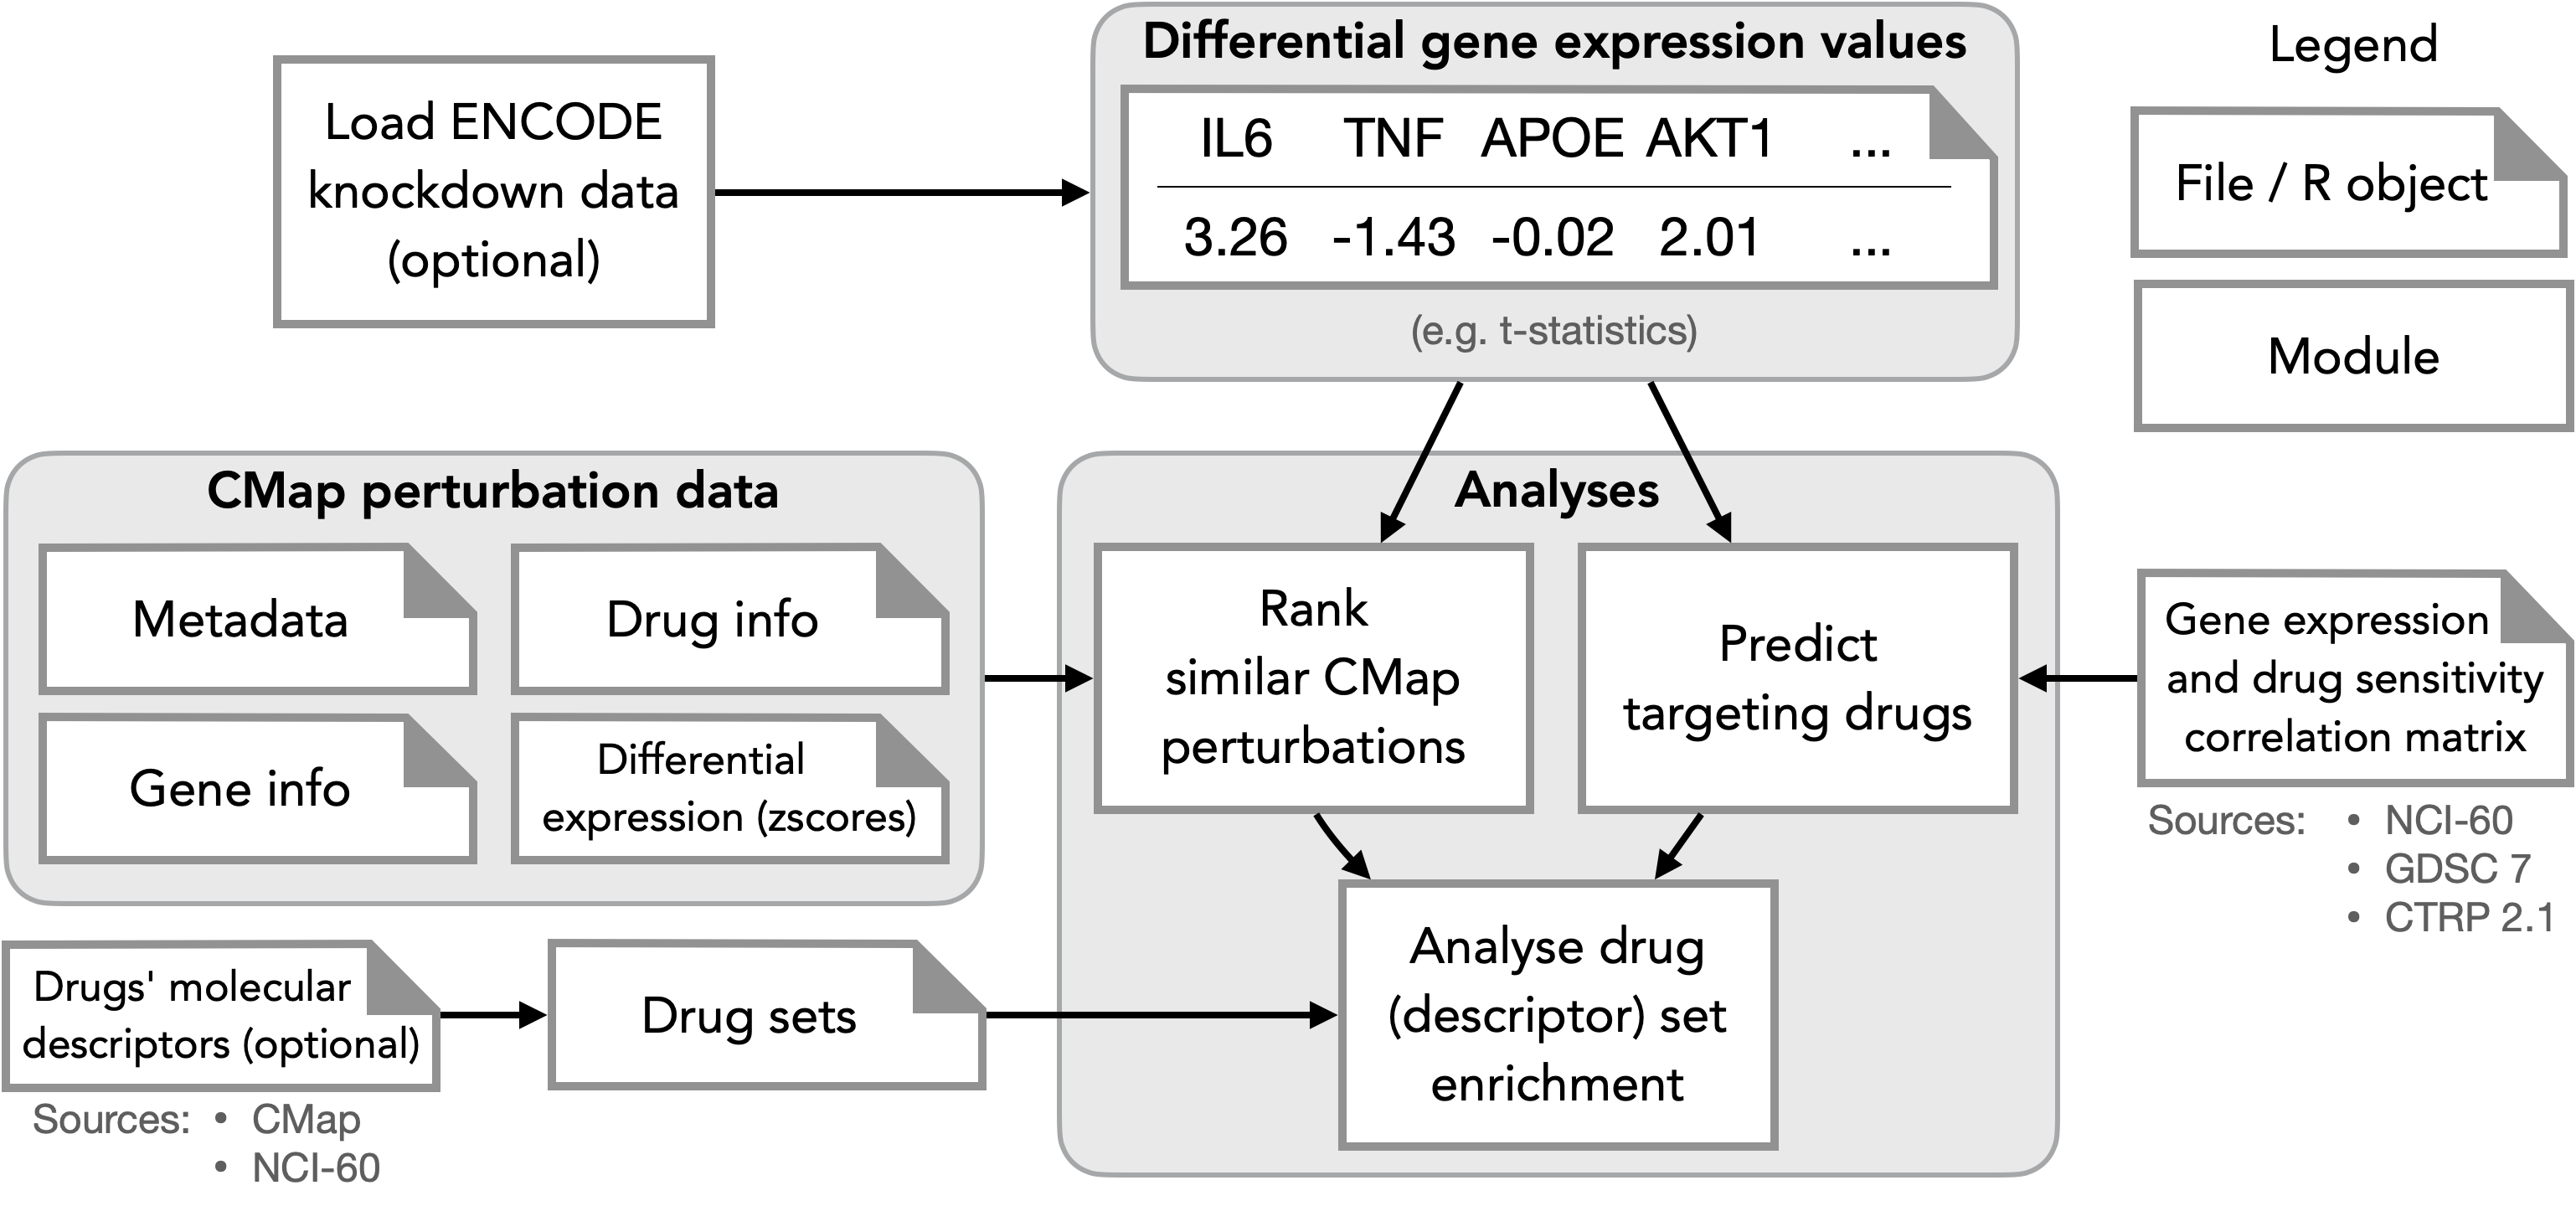
\includegraphics[width=.8\textwidth]{images/ctrap/workflow}
  \centering
  \caption[cTRAP workflow]{\textbf{cTRAP workflow.} cTRAP allows to perform three analyses: \textbf{(1) rank similar CMap perturbations} by comparing user-provided differential gene expression values against CMap perturbation data, \textbf{(2) predict targeting drugs} by comparing user-provided differential gene expression values against correlation matrices of gene expression and drug sensitivity data and \textbf{(3) analyse drug (descriptor) set enrichment} using drug sets and the results from either the first or second analysis. CMap perturbation data, gene expression/drug sensitivity correlation matrices and drug molecular descriptors for drug sets can be automatically downloaded.}
  \label{fig:ctrap-workflow}
\end{figure}

From a vector of user-provided differential expression results (e.g. t-statistic values) with respective gene symbols, cTRAP can return a ranked list of similar CMap perturbations or predict targeting drugs. Moreover, cTRAP can also analyse the enrichment of drug sets in an ordered vector of compounds to identify common compound characteristics (Figures \shorterref{fig:ctrap-workflow} and \shorterref{fig:ctrap-file-structure}).

\begin{figure}[!ht]
  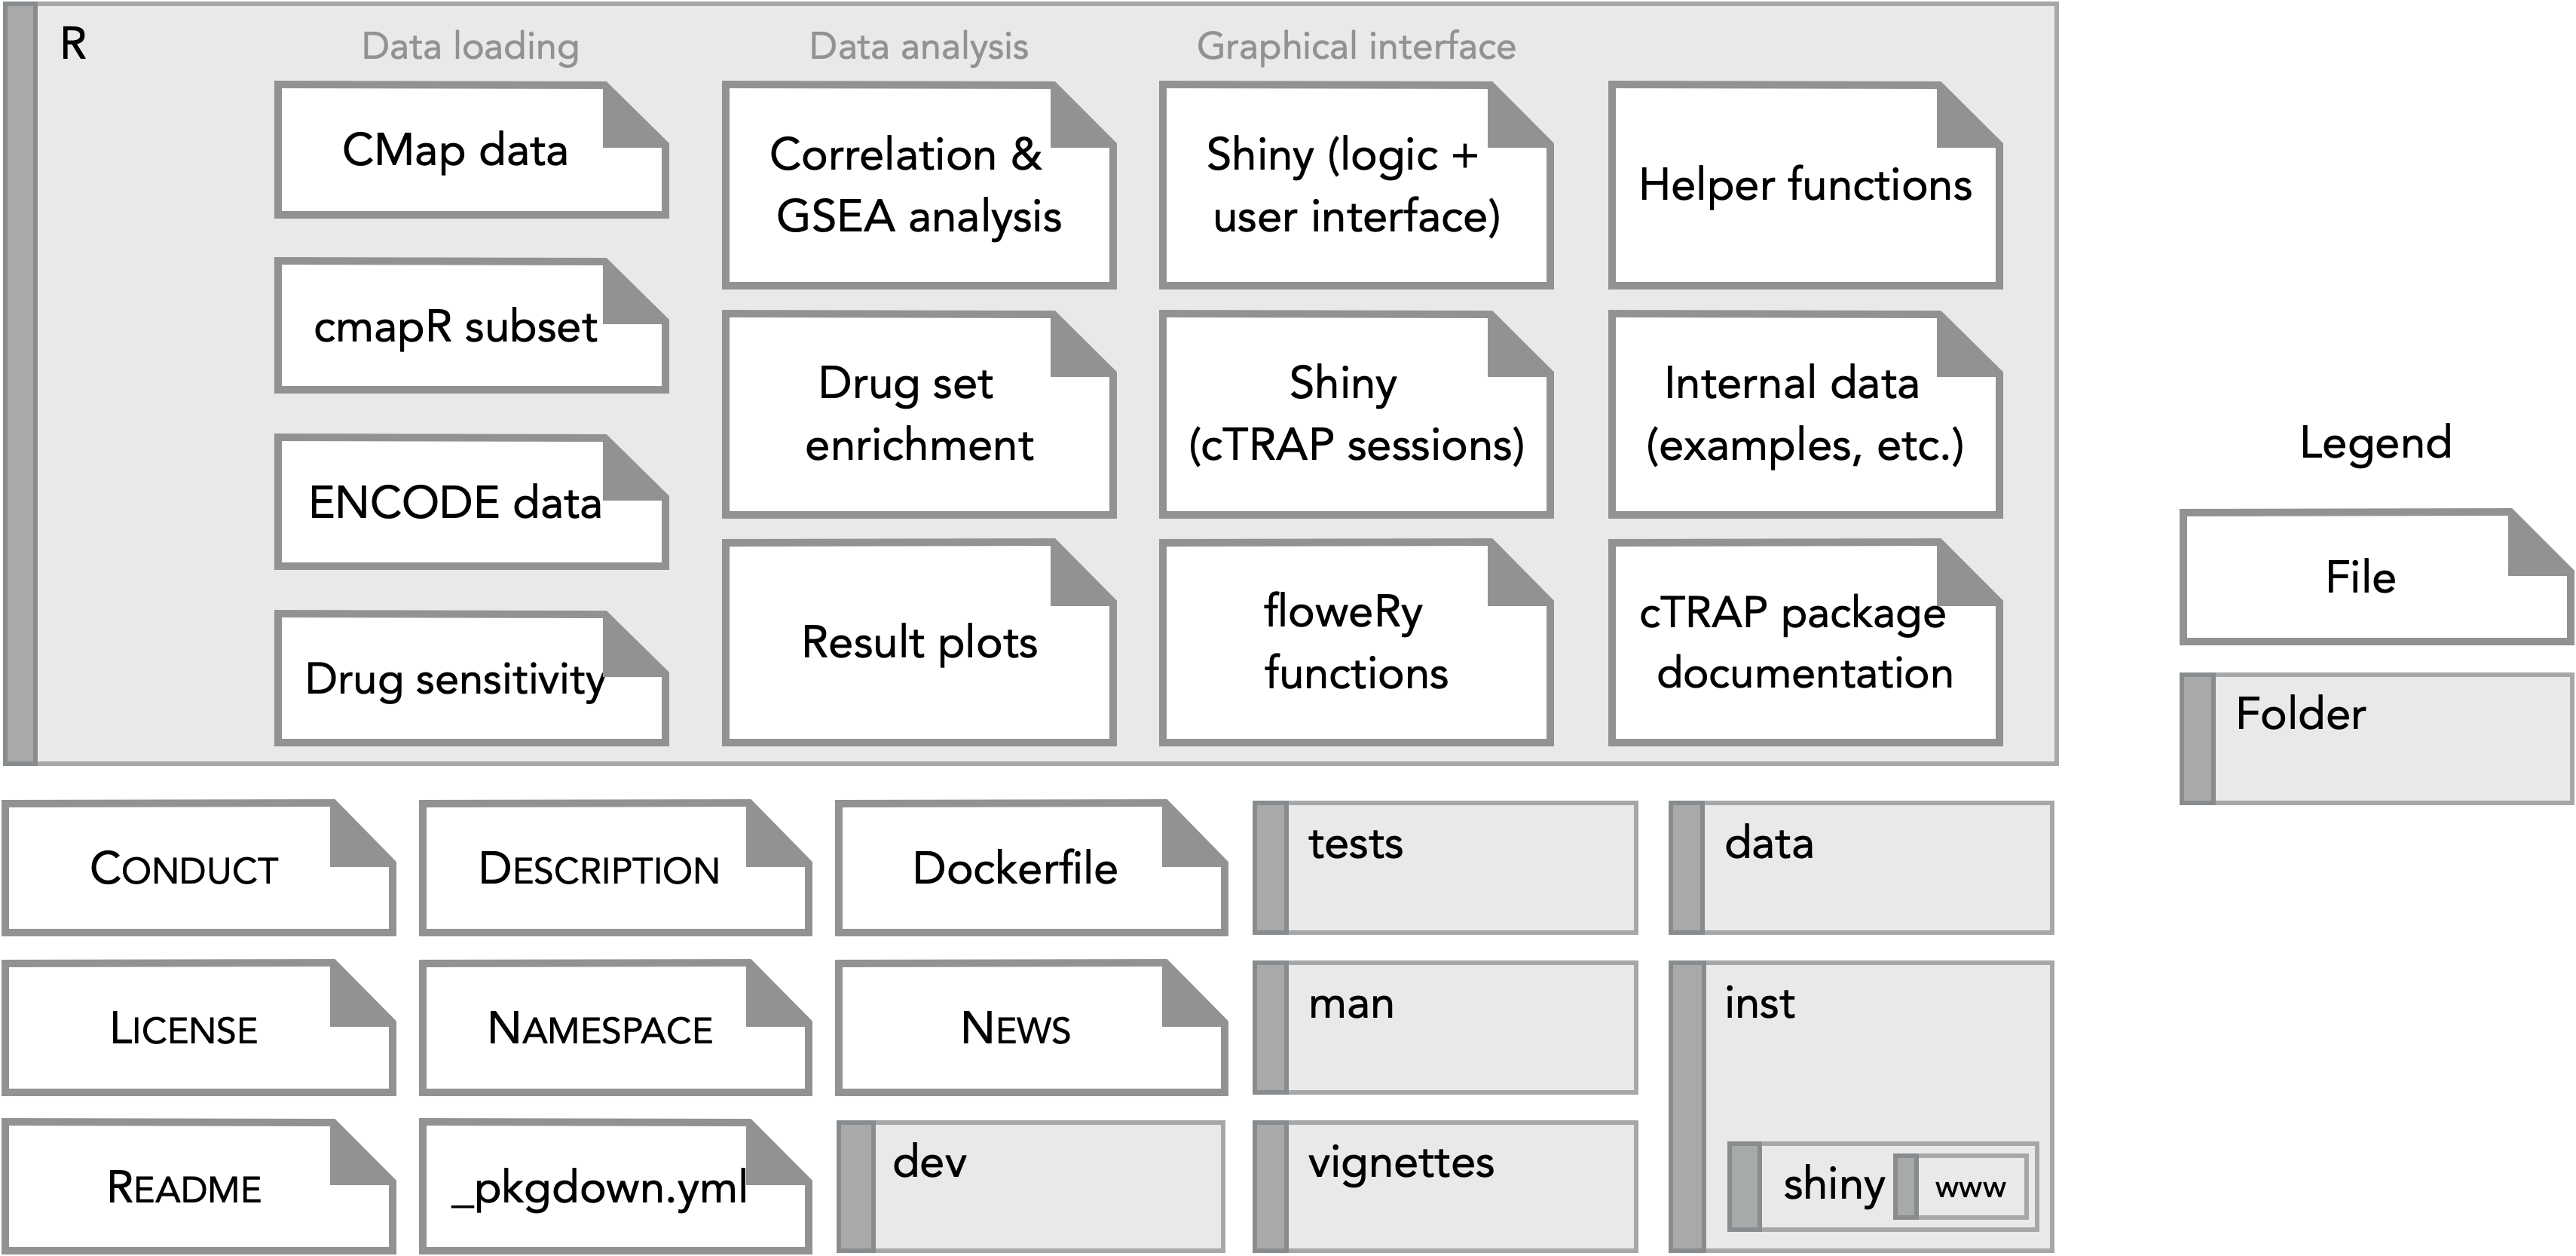
\includegraphics[width=1\textwidth]{images/ctrap/file-structure}
  \centering
  \caption[cTRAP file structure]{\textbf{Visual representation of cTRAP's file structure.} As usual in an R package, the \texttt{R} folder contains the scripts with cTRAP functions and data. \texttt{dev} is a custom folder that stores supporting scripts (e.g. test workflows and benchmarks); its contents are not included when building the R package.}
  \label{fig:ctrap-file-structure}
\end{figure}

\subsection{ENCODE knockdown data}

Using cTRAP, we can query and download ENCODE knockdown (and respective control) samples for multiple cell lines, filter low coverage counts from gene expression data, convert from ENSEMBL identifiers to gene symbol, and perform differential gene expression using \texttt{voom()}, \texttt{lmFit()} and \texttt{eBayes()} from the \texttt{limma} R package \cite{ritchie:2015tm}. First, \texttt{voom()} is used with the \emph{quantile} normalisation to transform count data to log\textsubscript{2} CPM (counts per million) and estimate the mean-variance relationship to compute weights used in linear modelling. Gene-wise linear models are then fitted using \texttt{lmFit()} between the knockdown and the control samples, followed by moderated t-tests and the calculation of log-odds of differential expression, using \texttt{eBayes()} for empirical Bayes moderation of standard errors.

cTRAP includes an example dataset (\texttt{diffExprStat}) with the differential gene expression results (t-statistic values) between the EIF4G1 knockdown in HepG2 versus control (\shortref{lst:diffExprStat}).

\begin{lstlisting}[caption=Code to obtain example dataset \texttt{diffExprStat}.,language=R,label={lst:diffExprStat}]
library(cTRAP)
ENCODEmetadata <- downloadENCODEknockdownMetadata(cellLine="HepG2",
                                                  gene="EIF4G1")
ENCODEsamples  <- loadENCODEsamples(ENCODEmetadata)[[1]]
counts         <- prepareENCODEgeneExpression(ENCODEsamples)

# Remove low coverage genes (>= 10 counts shared by >= 2 samples)
minReads   <- 10
minSamples <- 2
filter     <- rowSums(counts[ , -c(1, 2)] >= minReads) >= minSamples
counts     <- counts[filter, ]

# Convert ENSEMBL identifiers to gene symbols
counts$gene_id <- convertGeneIdentifiers(counts$gene_id)

# Perform differential gene expression (DGE) analysis
diffExpr <- performDifferentialExpression(counts)

# Get t-statistic values of DGE and respective gene names
diffExprStat <- diffExpr$t
names(diffExprStat) <- diffExpr$Gene_symbol
\end{lstlisting}

\subsection{Ranking of similar CMap perturbations}

\begin{figure}[!b]
  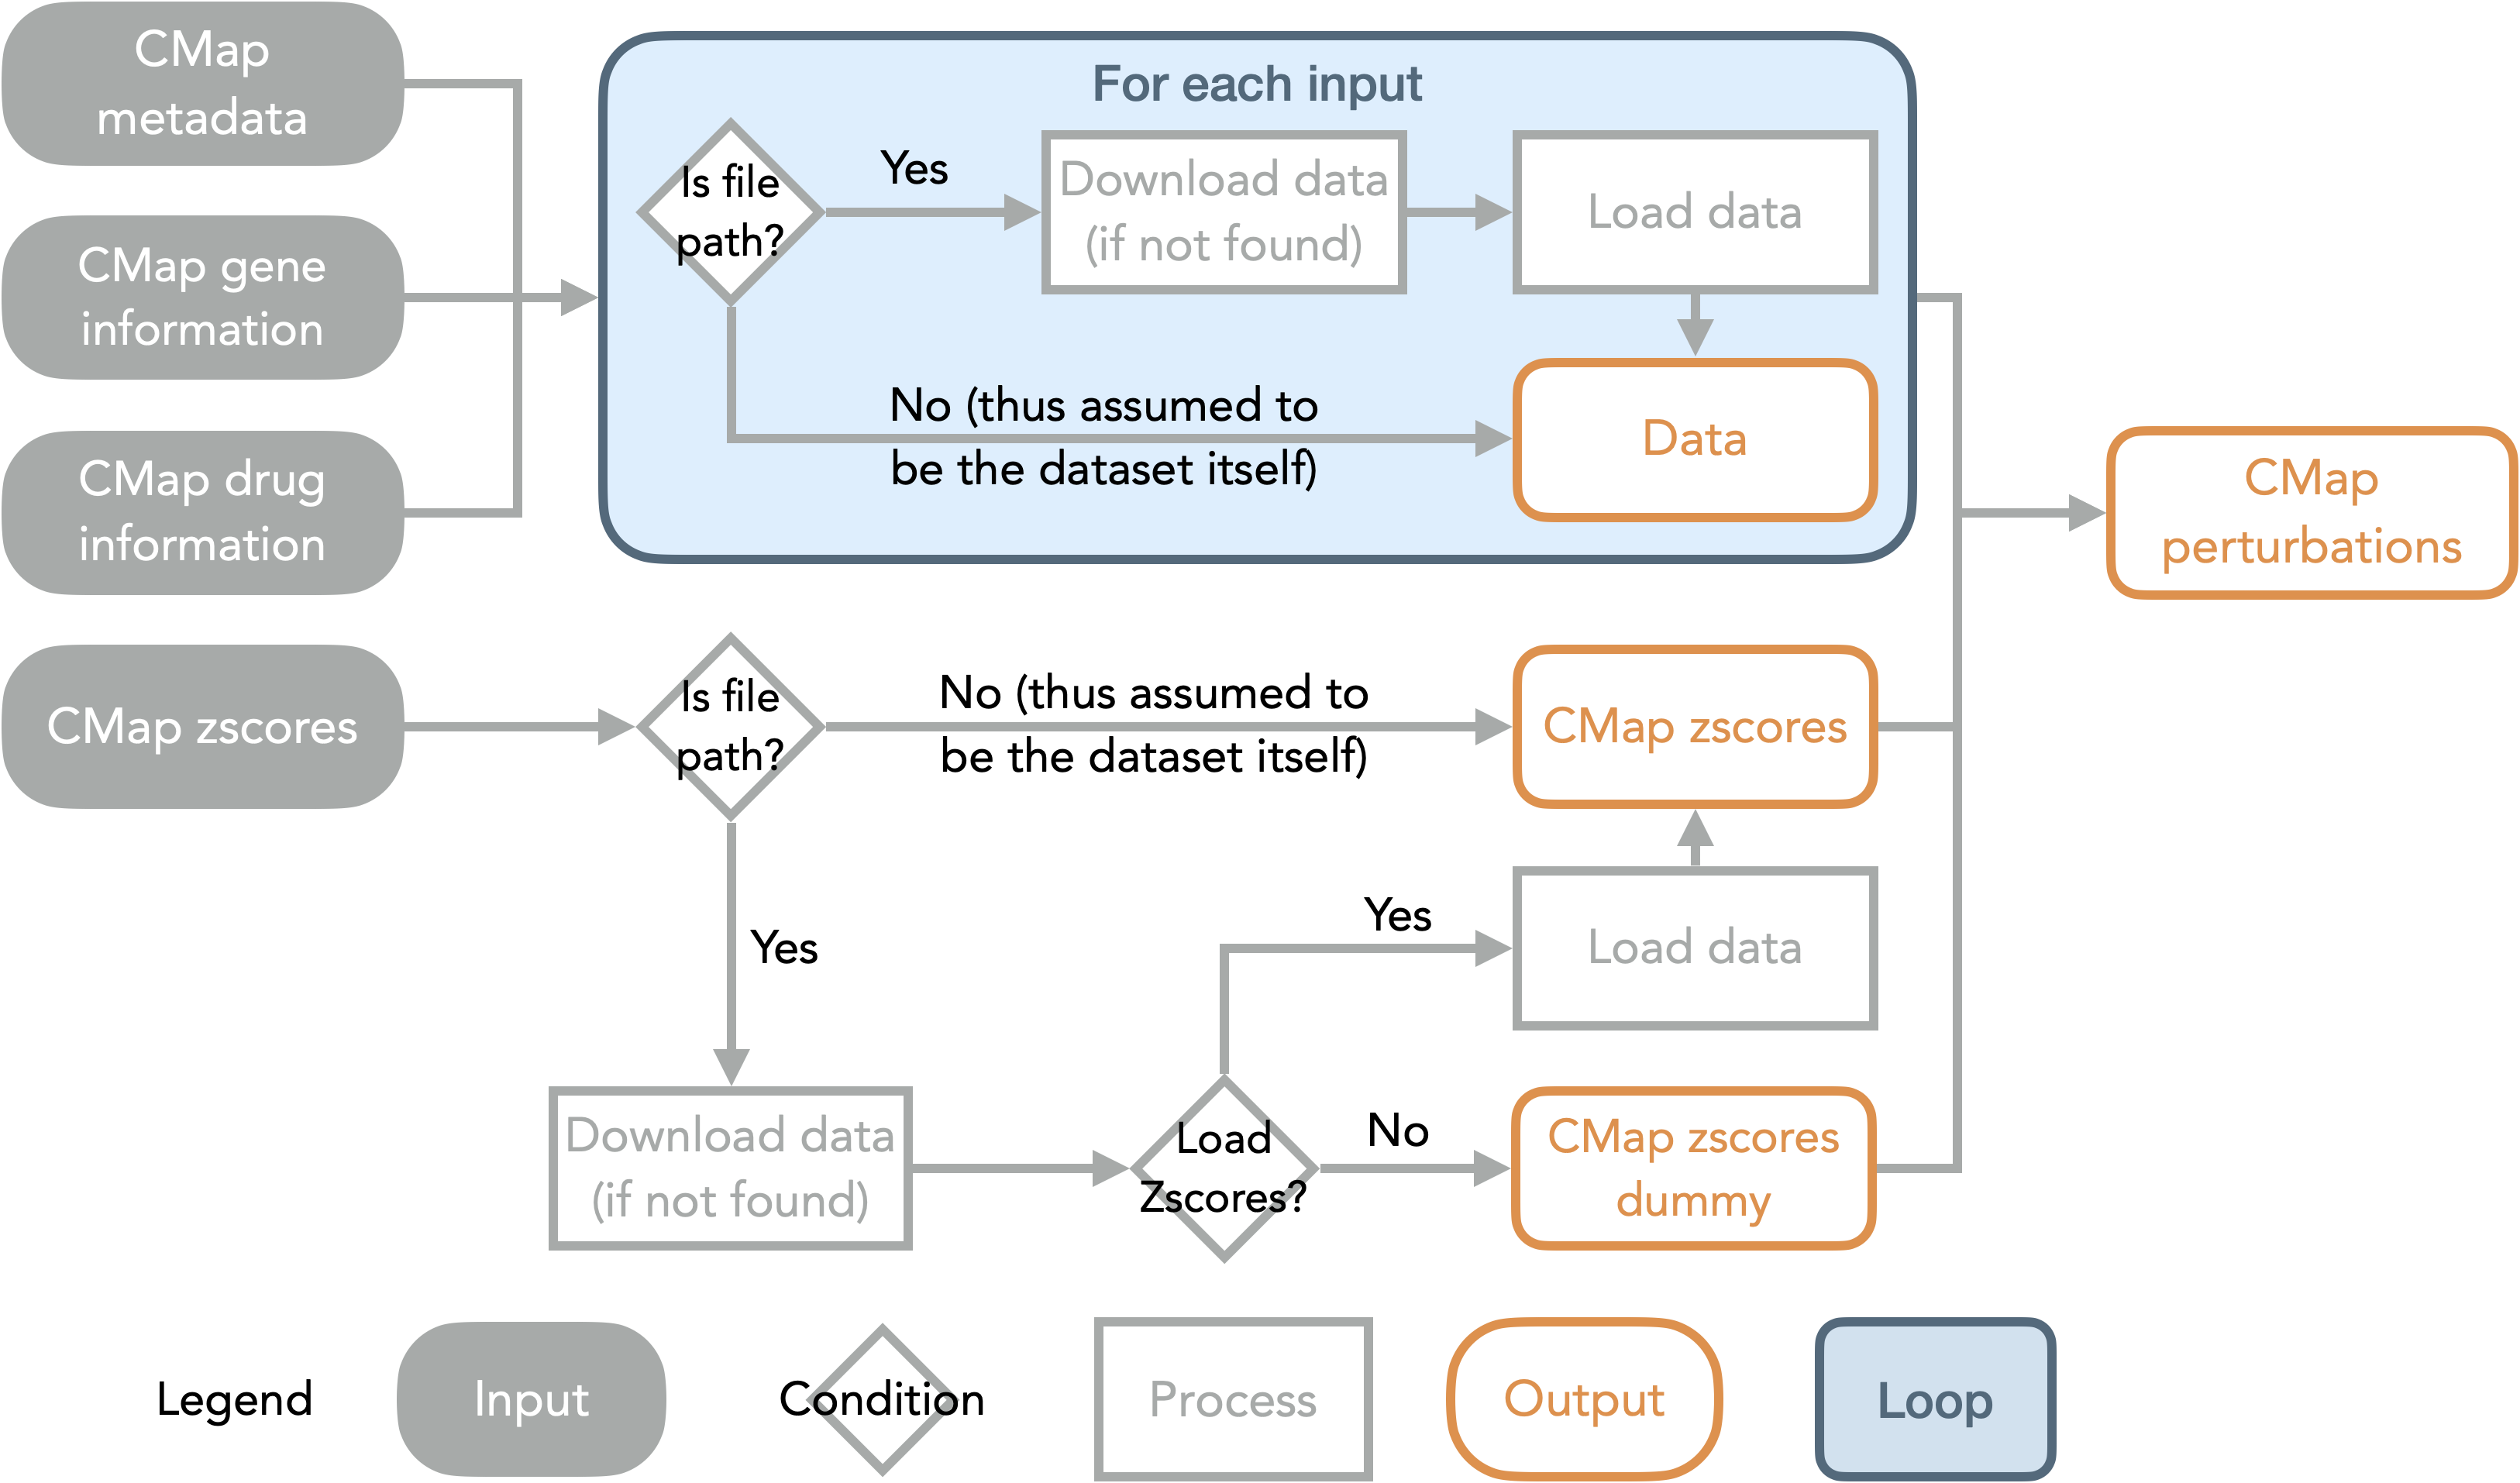
\includegraphics[width=.8\textwidth]{images/ctrap/cmap-perturbations}
  \centering
  \caption[Loading data from CMap perturbations]{\textbf{Loading data from CMap perturbations.} Input arguments support either the data itself (as data frames) or their respective file path. If the file path directs to a non-existing file,  data is first downloaded and then saved to the given file path. To avoid high memory usage, CMap perturbations' z-scores of differential expression profiles (CMap zscores) are not loaded into memory when a file path is given. Instead, only metadata are loaded into a \emph{dummy} object that can be subset as a normal R object for downstream analyses.}
  \label{fig:ctrap-cmap-perturbations}
\end{figure}

CMap perturbations can be categorised into gene knockdown, gene over-expression and compounds. In cTRAP, available perturbation types and respective conditions can be enquired using the function \texttt{getCMapConditions()} that will download CMap perturbation metadata. Afterwards, the function \texttt{filterCMapMetadata()} allows to filter the metadata based on selected perturbations types, cell lines, dosages and time points, allowing to specifically load only the desired data in downstream analyses. This information is passed to \texttt{prepareCMapPerturbations()} to download (if file is not found) and process CMap differential expression profiles z-scores (GCTX file) and gene and compound information (\shortref{fig:ctrap-cmap-perturbations}). Given that the GCTX file size is around 21GB, we recommend to download the file directly from GEO GSE92742’s Level 5 data link (\sloppy{\small{\url{ftp://ftp.ncbi.nlm.nih.gov/geo/series/GSE92nnn/GSE92742/suppl/GSE92742_Broad_LINCS_Level5_COMPZ.MODZ_n473647x12328.gctx.gz}}}).

After comparing differential expression z-scores from select CMap perturbations against user-provided differential expression results, \texttt{rankSimilarPerturbations()} returns a table with ranked CMap perturbations and their respective correlation coefficients and GSEA scores. Lower ranks indicate perturbations whose differential expression profiles are more similar to the user-provided data, i.e. CMap perturbations that potentially mimic the user-provided transcriptomic changes, whereas higher ranks define perturbations that may revert those changes.

To rank CMap perturbations, cTRAP performs Spearman's and Pearson's correlations between the user-provided statistics for differential expression and values from CMap perturbations, and calculates a GSEA-based score (all three methods are run by default). For each method, the similarity scores are averaged across multiple cell lines for the same conditions (when available) and those averages are then used to rank CMap perturbations. By default, results for individual cell lines are provided for informative purposes (e.g. to check the heterogeneity of response across cell lines) but not used when ranking. The different ranking scores are combined via the rank product, ultimately used to sort the CMap perturbations. % rank product not properly explained

The GSEA-based score is calculated via the following steps:

\begin{enumerate}
	\item Sort genes from the user-provided differential expression statistics;
	\item Define the top 150 (by default) and bottom 150 (by default) genes as two sets
	\item For each CMap perturbation, sort genes by their differential expression z-scores and calculate the Weighted Connectivity Score (WTCS) \cite{subramanian:2017ul} based on the GSEA enrichment scores for the two sets.
\end{enumerate}

As an example, for a CMap perturbation with a similar differential expression profile to user’s input, we expect to find higher enrichment of the top gene set in the most up-regulated genes and higher enrichment of the bottom gene set in the most down-regulated genes.

To minimise peak RAM usage, \texttt{prepareCMapPerturbations()} downloads the GCTX file (a customised HDF5 file) for the CMap’s perturbation differential expression z-scores (if not previously downloaded) and returns its path without loading the file content itself, creating a \emph{dummy} object that only stores its file path, perturbation names, gene symbols and other associated metadata (\shortref{fig:ctrap-cmap-perturbations}). Based on the file path of this \emph{dummy} object (that can be subset like a normal R object), \texttt{rankSimilarPerturbations()} loads a $\le$ 1 GiB chunk\footnote{The default 1 GiB ($1024^3$ bytes) allows loading chunks of around 10000 columns and 14000 rows ($10000 \times 14000 \times 8 \textrm{ bytes} / 1024^3 = 1.04 \textrm{ GiB}$). CMap's GCTX file has around 14000 rows (genes).}, compares its differential expression z-score values against user-provided data and repeats the analysis for the next chunk (\shortref{fig:ctrap-analyses}). For each chunk, multithreaded support for Linux and macOS can be enabled per comparison method via \texttt{parallel::mclapply()}\footnote{\texttt{mclapply()} parallelises tasks via forking where multiple child processes are spawned and share their parent's memory. Forking is unavailable in Windows and its alternatives were deemed unsatisfactory, given that they copy 1GiB chunks per thread, significantly slowing down runtime.}, enabled by setting the number of threads to 2 or higher.

\begin{figure}[!h]
  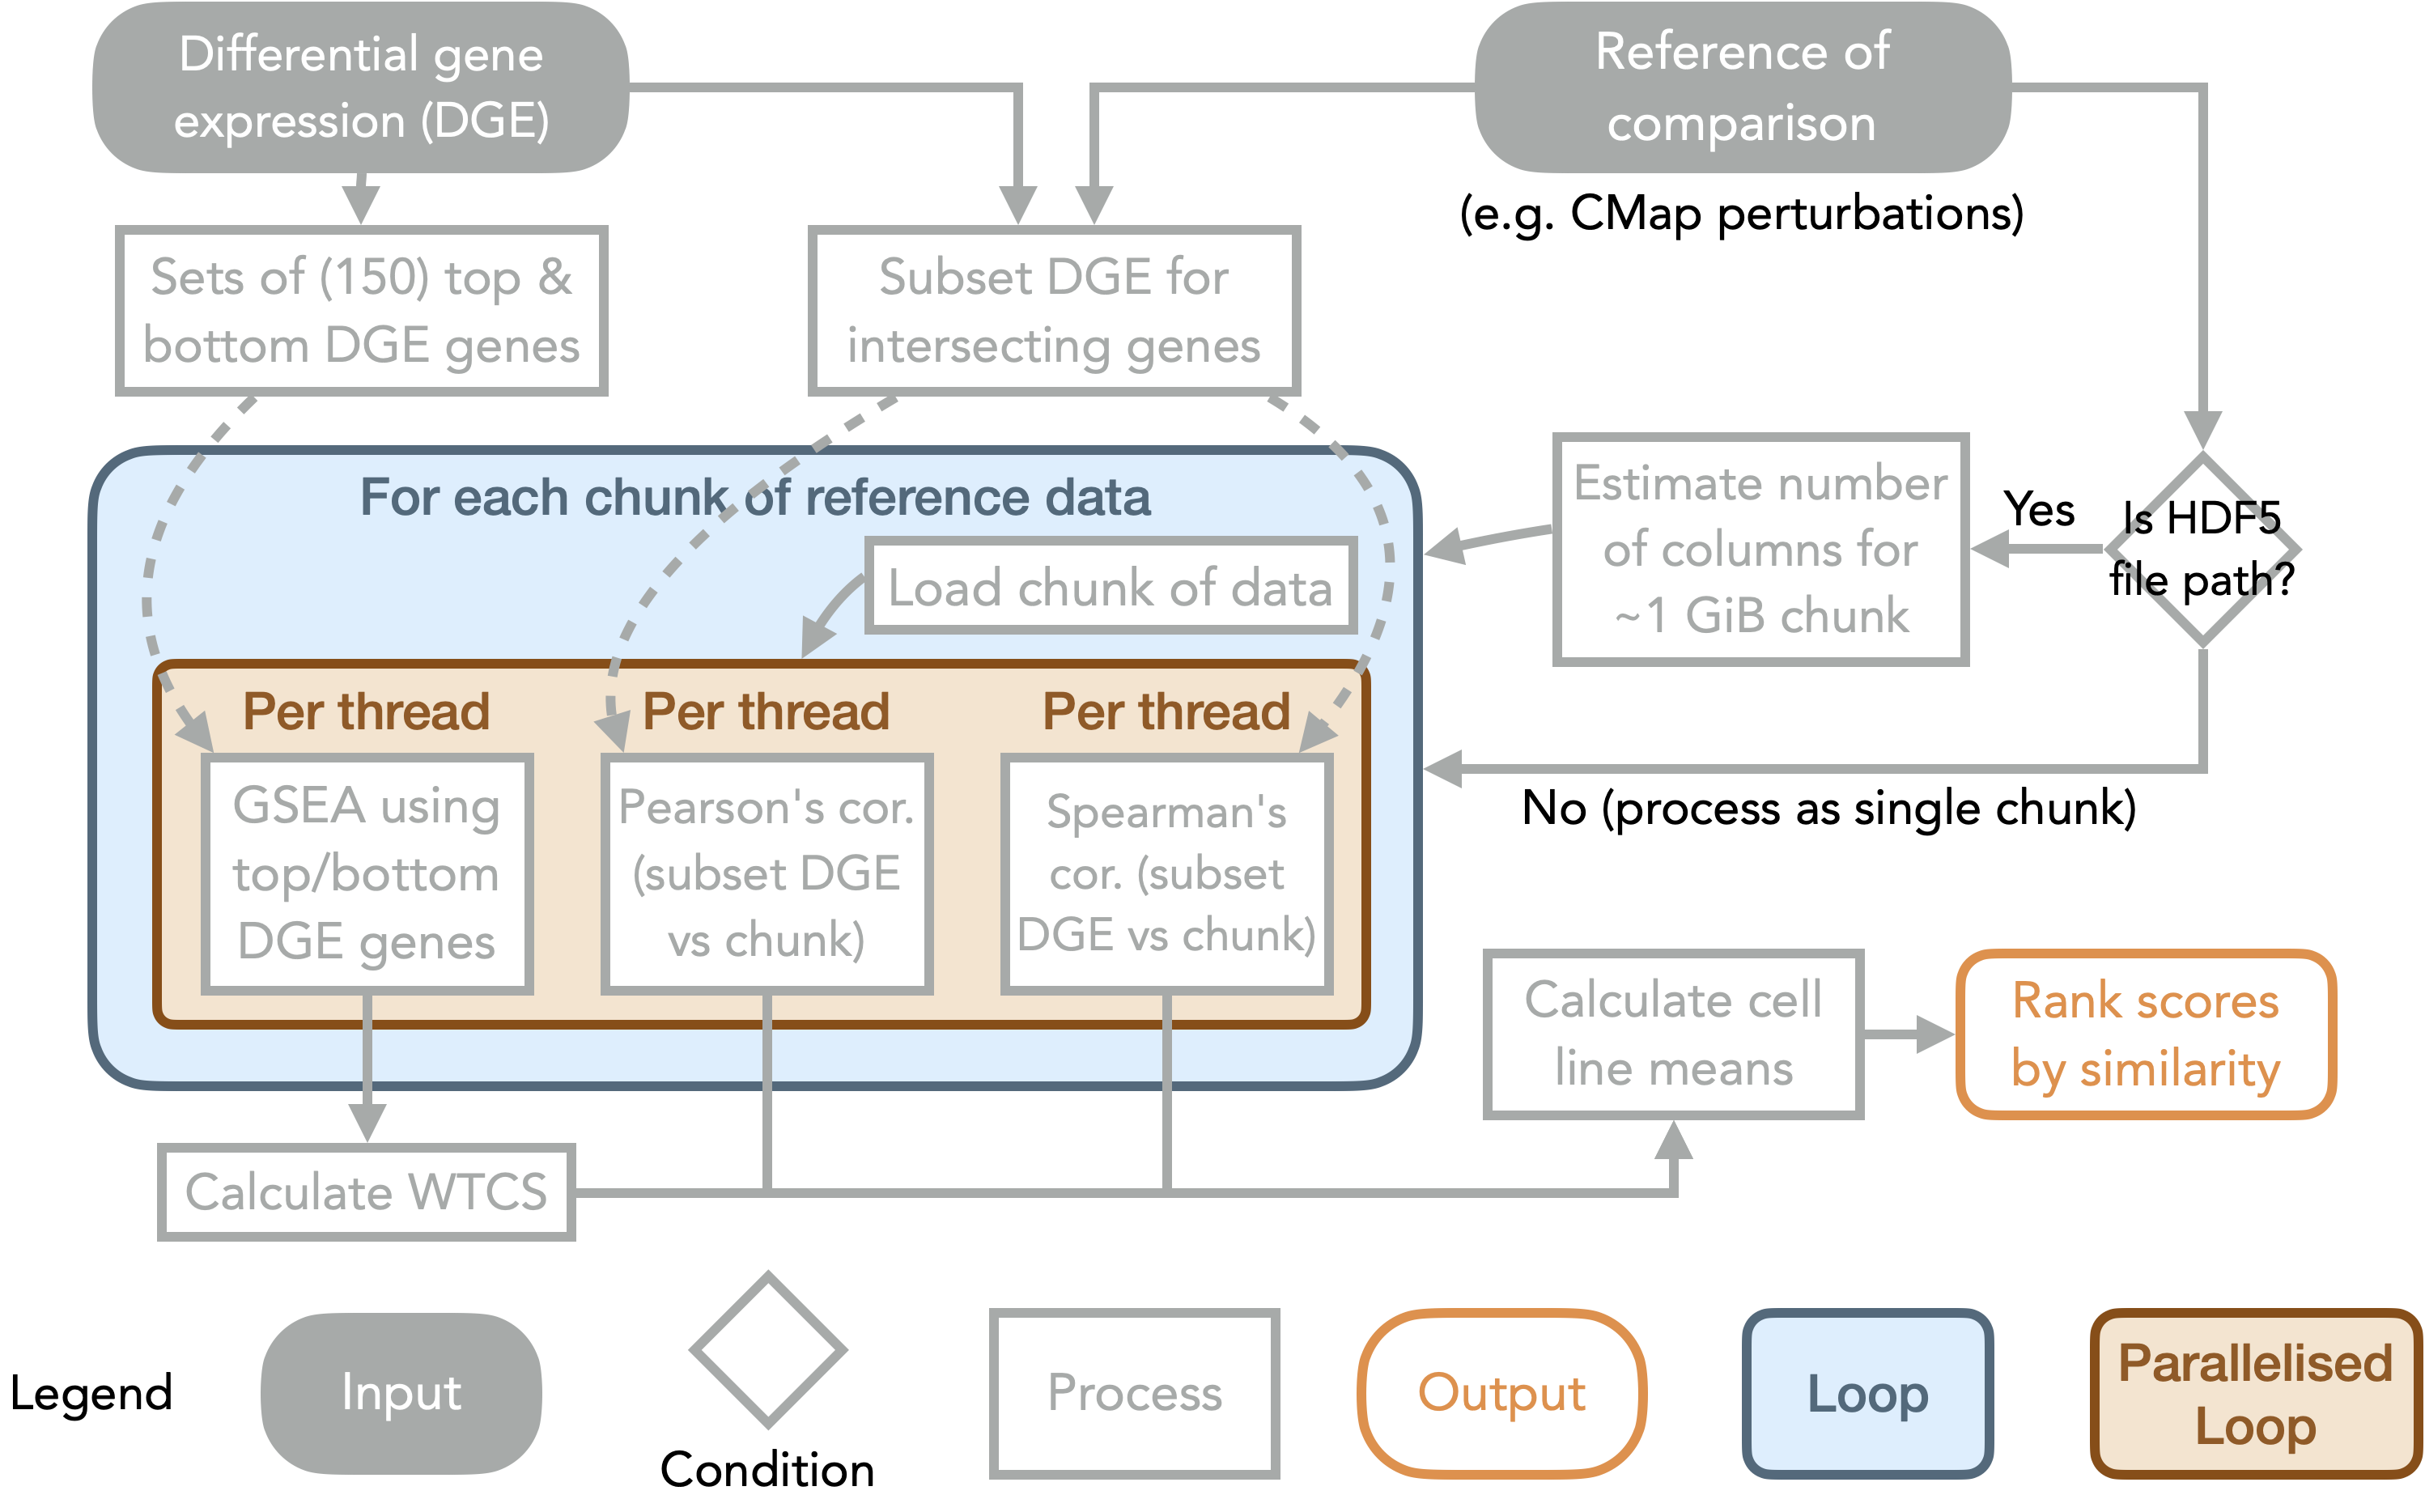
\includegraphics[width=.8\textwidth]{images/ctrap/analysis}
  \centering
  \caption[cTRAP similarity analysis]{\textbf{cTRAP similarity analysis.} User-provided differential gene expression is compared against a reference (e.g. differential expression z-scores of CMap perturbations) and ranked by similarity. If the reference of comparison is a HDF5 file path, the file is processed in 1GiB chunks to minimise peak memory usage. These analyses support multiple threads in Linux and macOS.}
  \label{fig:ctrap-analyses}
\end{figure}

The ranked list from \texttt{rankSimilarPerturbations()} can be plotted using \texttt{plot()}, showing a list of all results ordered by a given score or either a scatterplot or GSEA plot for a predicted targeting drug.

\subsection{Prediction of targeting drugs}

Gene expression and drug activity data across multiple cell lines are available from NCI-60 \cite{shoemaker:2006wi}, Cancer Therapeutics Response Portal (CTRP) 2.1 \cite{seashore-ludlow:2015ws} and Genomics of Drug Sensitivity in Cancer (GDSC) 7 \cite{yang:2012vk}. For each source, the internal function \texttt{prepareExpressionDrugSensitivityAssociation()} performs the following steps:

\begin{enumerate}
	\item Download all the necessary data depending on given source;
	\item Perform Spearman’s correlation (by default) between the expression of each gene against the sensitivity of intersecting cell lines to each drug;
	\item Generate a matrix with the correlation coefficients per gene and drug; and
	\item Prepare metadata for downstream analyses, including gene, compound and cell line information from each source.
\end{enumerate}

A higher correlation coefficient for a given gene and drug suggests a gene whose higher expression is associated with higher drug sensitivity across multiple cell lines. As this process can take multiple hours to finish for all sources, the resulting objects were stored online for each aforementioned source and can be listed with \texttt{listExpressionDrugSensitivityAssociation()} and downloaded and loaded into R using \texttt{loadExpressionDrugSensitivityAssociation()}.

To identify compounds that could target the phenotype associated with specific differential expression profiles, we use \texttt{predictTargetingDrugs()} with those profiles and a correlation matrix of gene expression and drug sensitivity as input. The correlation coefficients between gene expression and drug sensitivity for each drug are compared against user-provided differential expression results by Spearman’s and Pearson’s correlation and GSEA-based scores (as performed when ranking CMap perturbations, results from comparison methods are ranked and then those rankings are finally used to calculate the rank product’s rank). \texttt{predictTargetingDrugs()} returns a table with ranked predicted targeting drugs and their respective correlation coefficients and GSEA scores (\shortref{fig:ctrap-analyses}). A lower rank comprise drugs that may target phenotypes similar to the user-provided differential expression profile.

The resulting object can be plotted with \texttt{plot()}, showing a list of all results ordered by a given score or either a scatterplot or GSEA plot for a predicted targeting drug. The function \texttt{plotTargetingDrugsVSsimilarPerturbations()} compares the results from predicted targeting drugs and CMap perturbations that may mimic or revert the observed phenotype. For the available compound identifiers in the metadata pertaining from the different datasets (e.g. compound name, Broad ID, PubChem CID and SMILES), the function will automatically select the identifiers with higher number of matching values between the two datasets, unless the identifiers are explicitly defined by the user. A scatterplot is then returned using, by default, the rank product’s rank of targeting drugs against the rank product’s rank of similar perturbations.

\subsection{Drug descriptor set enrichment analysis}

Juan Carlos, a former member of the lab, computed drug descriptors (e.g. molecular weight and number of aromatic rings) for compounds from CMap and NCI-60 based on their three-dimensional (3D) and two-dimensional (2D) characteristics. These descriptors were uploaded to \alink{compbio.imm.medicina.ulisboa.pt/public/cTRAP/} and the resulting files can be automatically downloaded and processed to R using \texttt{loadDrugDescriptors()}.

\texttt{prepareDrugSets()} allows to create sets of descriptors. By default, the function creates a maximum of 15 sets per drug descriptor. For each alphanumeric descriptor, one set is created per unique value of that descriptor. Alphanumeric descriptors containing more than 15 unique values (by default) will be discarded. For numerical descriptors, \texttt{prepareDrugSets()} internally uses the \texttt{binr::bins()} function to create evenly-distributed bins of drug descriptors, where each set contains a minimum number of points equal to the number of non-missing values divided by the number of maximum sets (15 by default) divided by a constant (5 by default).

The \texttt{analyseDrugSetEnrichment()} function analyses the enrichment of the created drug descriptor sets in a named numeric vector or an object returned from \texttt{rankSimilarPerturbations()} – only if run against CMap compound perturbations – or \texttt{predictTargetingDrugs()}. The GSEA-based enrichment analysis is internally performed using \texttt{fgsea::fgsea()}. The resulting object can be plotted with \texttt{plot()}, showing a list of all results ordered by a given score or either a scatterplot or GSEA plot for a predicted targeting drug.

\subsection{Time and memory benchmarking}

We measured elapsed time using R’s \texttt{Sys.time()} immediately before and after ranking similar CMap perturbations, predicting targeting drugs (using NCI60 expression and drug sensitivity association, the most time-consuming option) and performing drug set enrichment analysis using a development version of cTRAP 1.10 (commit \link{https://github.com/nuno-agostinho/cTRAP/commit/296f9b2}{296f9b2} from January 2022). As input, we used the t-statistics for the differential expression between EIF4G1 knockdown versus control based on ENCODE gene expression data from cell line HepG2 (\texttt{cTRAP::diffExprStat} object).

Using the same input, we measured heap memory usage of cTRAP 1.10 dev (\link{https://github.com/nuno-agostinho/cTRAP/commit/296f9b2}{296f9b2}) while ranking CMap perturbations when running R 4.0.3 in debug mode with heaptrack 1.0.0\footnote{heaptrack is an open-source memory allocation profiler available at \alink{github.com/KDE/heaptrack}}. For R to work properly with heaptrack, the \path{/usr/bin/R} file was edited -- all lines of the last \emph{if} statement were commented out, except for:

\begin{lstlisting}[language=bash,numbers=none]
exec ${debugger} ${debugger_args} "${R_binary}" ${args} "${@}"
\end{lstlisting}

Afterwards, we benchmarked the memory usage while running cTRAP with:

\begin{lstlisting}[language=bash,numbers=none]
R -d heaptrack -f ${cTRAP_Rscript} --args ${cTRAP_Rscript_args}
\end{lstlisting}

All benchmarks were run in a workstation with Ubuntu 18.04.5 LTS, 768 GB of RAM memory and 72 cores (Intel Xeon Gold 6254 CPU @ 3.10GHz). The benchmark scripts are open-source and describe how to profile time and memory in cTRAP and plot subsequent results: \alink{github.com/nuno-agostinho/cTRAP/tree/master/dev/benchmark}.

\subsection{Continuous integration}

Akin to psichomics (\fullref{subsec:psichomics-ci}), GitHub Actions are used with cTRAP to update its Docker images in Docker Hub (\dockerlink{nunoagostinho/ctrap}) and GitHub (\alink{github.com/nuno-agostinho/cTRAP}); update website documentation via \texttt{roxygen} \cite{wickham:2021wt} and \texttt{pkgdown} \cite{wickham:2021wj}; and check for errors and warnings when building cTRAP in Windows, macOS and Linux.

\section{Results}

cTRAP's web app is available at \alink{compbio.imm.medicina.ulisboa.pt/cTRAP}. Alternatively, users can install cTRAP in their own computers, allowing them to use local computing resources. Similarly to psichomics, cTRAP offers both graphical and command-line interfaces. Although most features are common to both interfaces, we recommend less experienced users to opt for the Shiny-based graphical interfaces.

\subsection{Case study}

For this case study, we used RNA-seq data from EIF4G1 shRNA knockdown experiments in HepG2 cell line from the ENCODE project. The RNA-seq processed data (gene quantifications from RSEM method) for the EIF4G1 knock-down and respective controls (two replicates each) was automatically downloaded by cTRAP.

\subsubsection{Differential gene expression analysis of ENCODE RNA-seq data}

Gene expression data (read counts) were quantile-normalized using voom, followed by differential expression analysis performed using \texttt{limma} \cite{ritchie:2015tm}. We used the respective t-statistic as our metric of differential expression to compare with CMap’s gene knock-down perturbations in the same cell line (HepG2)\footnote{This comparison could also be done to perturbations in a different cell line (or in all cell lines using the average result across cell lines).}.

% To summarise conditions and check available data in CMap, we can use the following commands to download CMap metadata:

Afterwards, we filtered the metadata to CMap gene knockdown perturbations in HepG2 and loaded associated gene information and differential gene expression data based on the given filename. The differential gene expression z-scores from CMap were also loaded for small molecule perturbations.

Differential gene expression data for each CMap perturbation are available in normalised z-score values \cite{subramanian:2017ul}.

\subsubsection{Comparison with CMap perturbations}

The \texttt{rankSimilarPerturbations()} function compares the differential expression metric (the t-statistic, in this case) against the CMap perturbations’ z-scores using the available methods:

\begin{itemize}
    \item Spearman’s correlation
    \item Pearson’s correlation
    \item Gene Set Enrichment Analysis (GSEA), where the most up- and down-regulated n genes from the user’s differential expression profile are used as gene sets (by default, $n = 150$ genes)
\end{itemize}

The output table contains the results of the comparison with each perturbation tested, including the test statistics (Spearman’s correlation coefficient, Pearson’s correlation coefficient and/or GSEA score), the respective p-value and the Benjamini-Hochberg-adjusted p-value (for correlation statistics only). When performing multiple methods, the rank product’s rank will be included to summarise other method’s rankings.

The Gene Set Enrichment Analysis (GSEA) score is based on the Weighted Connectivity Score (WTCS), a composite and bi-directional version of the weighted Kolmogorov-Smirnov enrichment statistic (ES) \cite{subramanian:2017ul}. To calculate the GSEA score, GSEA is run for the most up- and down-regulated genes from the user’s differential expression profile. The GSEA score is the mean between EStop and ESbottom (however, if EStop and ESbottom have the same sign, the GSEA score is 0).

If a perturbation has a similar differential expression profile to our data (higher GSEA score), we expect to see the most up-regulated (down-regulated) genes in the perturbation enriched in the top (bottom) n differentially expressed genes from our data.

To analyse the relationship between the user-provided differential expression profile with that associated with a specific perturbation, scatter plots (for Spearman and Pearson analyses) and GSEA plots are available.

For instance, let’s plot the relationship between EIF4G1 shRNA knockdown from ENCODE with the CMap knockdown perturbations.

\subsubsection{Predicted targeting drugs}

Compounds that target the phenotypes associated with the user-provided differential expression profile can be inferred by comparing against gene expression and drug sensitivity associations. The gene expression and drug sensitivity datasets derived from the following sources were correlated using Spearman’s correlation across the available cell lines.

\begin{wraptable}{r}{7cm}
\centering
\parnotereset
\small
\caption[Drug sensitivity datasets statistics]{\textbf{Drug sensitivity datasets statistics.} Number of screened compounds and human cancer cell lines.}
\label{tab:drug-sensitivity-datasets}
\begin{tabularx}{.47\textwidth}{ l r r }
\toprule
\textbf{Source}   & \textbf{Compounds} & \textbf{Cell lines} \\
\midrule
NCI60             &                   $>$ 100 000 & 60 \\
GDSC 7            &                           481 & 860 \\
CTRP 2.1          &                           138 & $\sim$ 700 \\
\bottomrule
\end{tabularx}
\parnotes
\end{wraptable}

To use an expression and drug sensitivity association based on CTRP 2.1 (GDSC 7 and NCI60 could be used instead) to infer targeting drugs for the user’s differential expression profile.

Compounds are ranked by their relative targeting potential based on the input differential expression profile (i.e. the 1st-ranked compound has higher targeting potential than the 2nd-ranked one).

Candidate targeting drugs were plotted against the similarity ranking of their perturbations towards the user’s differential expression profile. Note that the highlighted values are the same compounds for the following plots annotated with their name, gene target and mechanism of action (MOA), respectively.

\subsubsection{Molecular descriptor enrichment analysis}

Using our candidate targeting drugs, we analysed the enrichment of 2D and 3D molecular descriptors based on CMap and NCI60 compounds. Our list of targeting drugs is particularly enriched in specific drug descriptors that allows us think about the relevance of these descriptors for targeting a phenotype of interest.

\subsection{Time and memory optimisation}
\label{subsec:ctrap-optim}

cTRAP allows comparing user-provided differential expression results against those from CMap perturbations that is loaded based on their public data, including a 21GB GCTx file containing the CMap perturbation z-scores. The GCTX format stores annotated, high-dimensional data matrices and is based on the HDF5 format for efficient indexing and loading of subsets of the whole data \cite{enache:2018wq}. Instead of loading the whole GCTx file into memory, cTRAP 1.4 and newer minimises peak RAM usage by loading and processing subsets of perturbation z-scores in one of two ways:

\begin{itemize}
	\item Load and process selected perturbations only (e.g. compound perturbations), avoiding loading perturbations that will not be compared.
	\item Load and process selected perturbations by 1 GiB chunks (default).
\end{itemize}

Although the concept of processing by chunks helped reducing the memory footprint of cTRAP, we later refactored the code of the comparisons in cTRAP 1.10, a milestone that included multiple improvements to speed and memory:

\begin{itemize}
	\item Faster GSEA-based score calculation by improving code efficiency.
	\item Slightly improved runtime by avoiding redundant loading of data chunks. This change was also required to enable multi-thread support in systems that support process forking (e.g. Linux and macOS, but not Windows).
	\item Optional argument to set a custom size for data chunks (1 GiB by default).
	\item As the NCI60 gene expression and drug sensitivity correlation matrix is also big (3.3GB), we saved that matrix as a HDF5 file that is then loaded and processed by cTRAP in chunks of 1 GiB (by default), minimising peak RAM usage when predicting targeting drugs based on the NCI60 data.
\end{itemize}

We benchmarked time and memory when ranking CMap perturbations based on Spearman's correlation, Pearson's correlation and GSEA-based score using a development version of cTRAP 1.10 (commit \link{https://github.com/nuno-agostinho/cTRAP/commit/296f9b2}{296f9b2}) and using the t-statistics for differential expression between EIF4G1 knockdown versus control based on ENCODE gene expression data from HepG2 cell line as input. The number of CMap compound perturbations (241 258) is much higher than the knockdown (48 862) and over-expression (24 627) perturbations and this is expected to reflect on time and memory for data processing.

\begin{figure}[!b]
  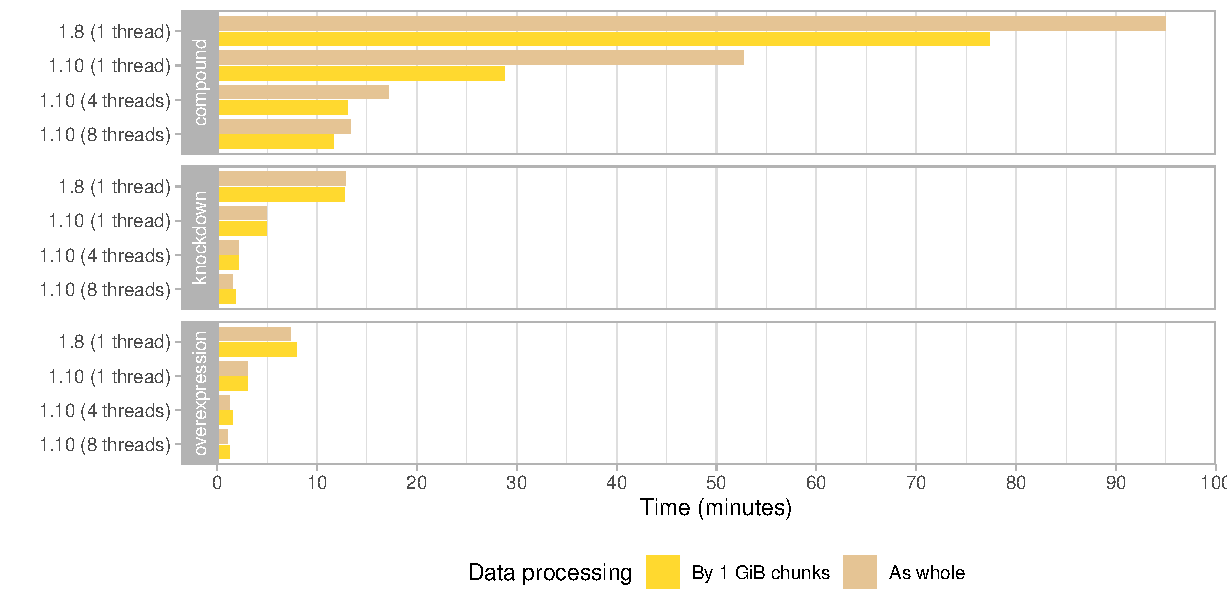
\includegraphics[width=\textwidth]{images/ctrap/ranking-time}
  \centering
  \caption[Time benchmark of CMap perturbation ranking]{\textbf{Time benchmark of CMap perturbation ranking.} Times were measured for cTRAP 1.8 (1 thread only) and 1.10 (1, 4 and 8 threads) for over-expression, knockdown and compound perturbations whose data was loaded by 1 GiB chunks or as whole.}
  \label{fig:cmap-ranking-time}
\end{figure}

When ranking CMap compound perturbations in cTRAP 1.8 and 1.10, the runtime was decreased from 95 to 53 minutes when loading the whole data and from 77 to 28 minutes when loading by chunks (\autoref{fig:cmap-ranking-time}). For each chunk, we parallelised the calculations performed per perturbation and it can help to speed up runtime comparing against CMap compound perturbations with 4 threads from 28 to 12 minutes. However, the usage of 8 threads is not recommended as the runtime is similar to using 4 threads while consuming the double number of threads.

Benchmarked memory was annotated based on the different internal steps performed by cTRAP (\autoref{fig:cmap-ranking-memory}). When ranking against the CMap compound perturbations, loading and processing their z-scores at once requires 59.7 GiB, compared to 5.4 GiB when loading and processing 1 GiB chunks. The differences were not as stark when using the knockdown and over-expression perturbations, but were still crucial to allow the possibility of running cTRAP in a common laptop with 8 GiB of RAM. % Although memory profiling expectedly slows down runtime, we can also see in the memory benchmark that loading data by chunks can have a big impact on elapsed time of a run when comparing compound perturbations.

\begin{figure}[!ht]
  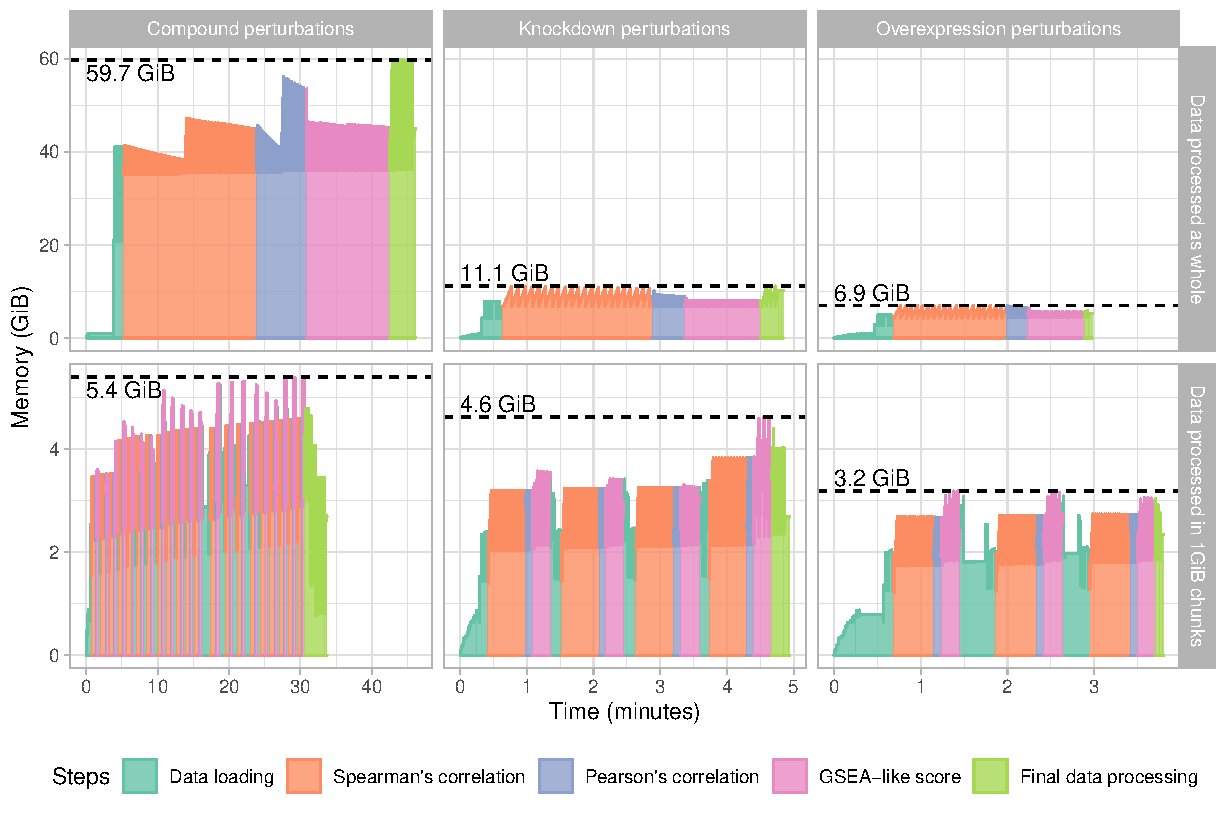
\includegraphics[width=\textwidth]{images/ctrap/ranking-memory}
  \centering
  \caption[Memory benchmark of CMap perturbation ranking]{\textbf{Memory benchmark of CMap perturbation ranking,} annotated using the different steps performed by cTRAP. Memory was benchmarked when ranking compound, knockdown and overexpression perturbations against differential expression results. The maximum memory for each condition is labelled.}
  \label{fig:cmap-ranking-memory}
\end{figure}

\subsection{Graphical interface}

To assist users that may prefer graphical interfaces, most cTRAP functionality is exposed via 5 modular and independent functions that launch web apps (\autoref{fig:ctrap-ui-functions}):

\begin{itemize}
	\item \texttt{launchDiffExprLoader()} to load differential expression data. Returns a differential expression object that can be used in cTRAP analyses.
	\item \texttt{launchCMapDataLoader()} to explore and load CMap data by type of perturbation, cell types, time points and dosages. Returns filtered CMap data based on the user's selection.
	\item \texttt{launchMetadataViewer()} to check metadata of given cTRAP objects.
	\item \texttt{launchResultPlotter()} to view and plot cTRAP results given as input.
	\item \texttt{launchDrugSetEnrichmentAnalyser()} to analyse drug set enrichment and visualize respective results.
\end{itemize}

\begin{figure}[!h]
	\centering
	\begin{subfigure}[h]{0.3\textwidth}
		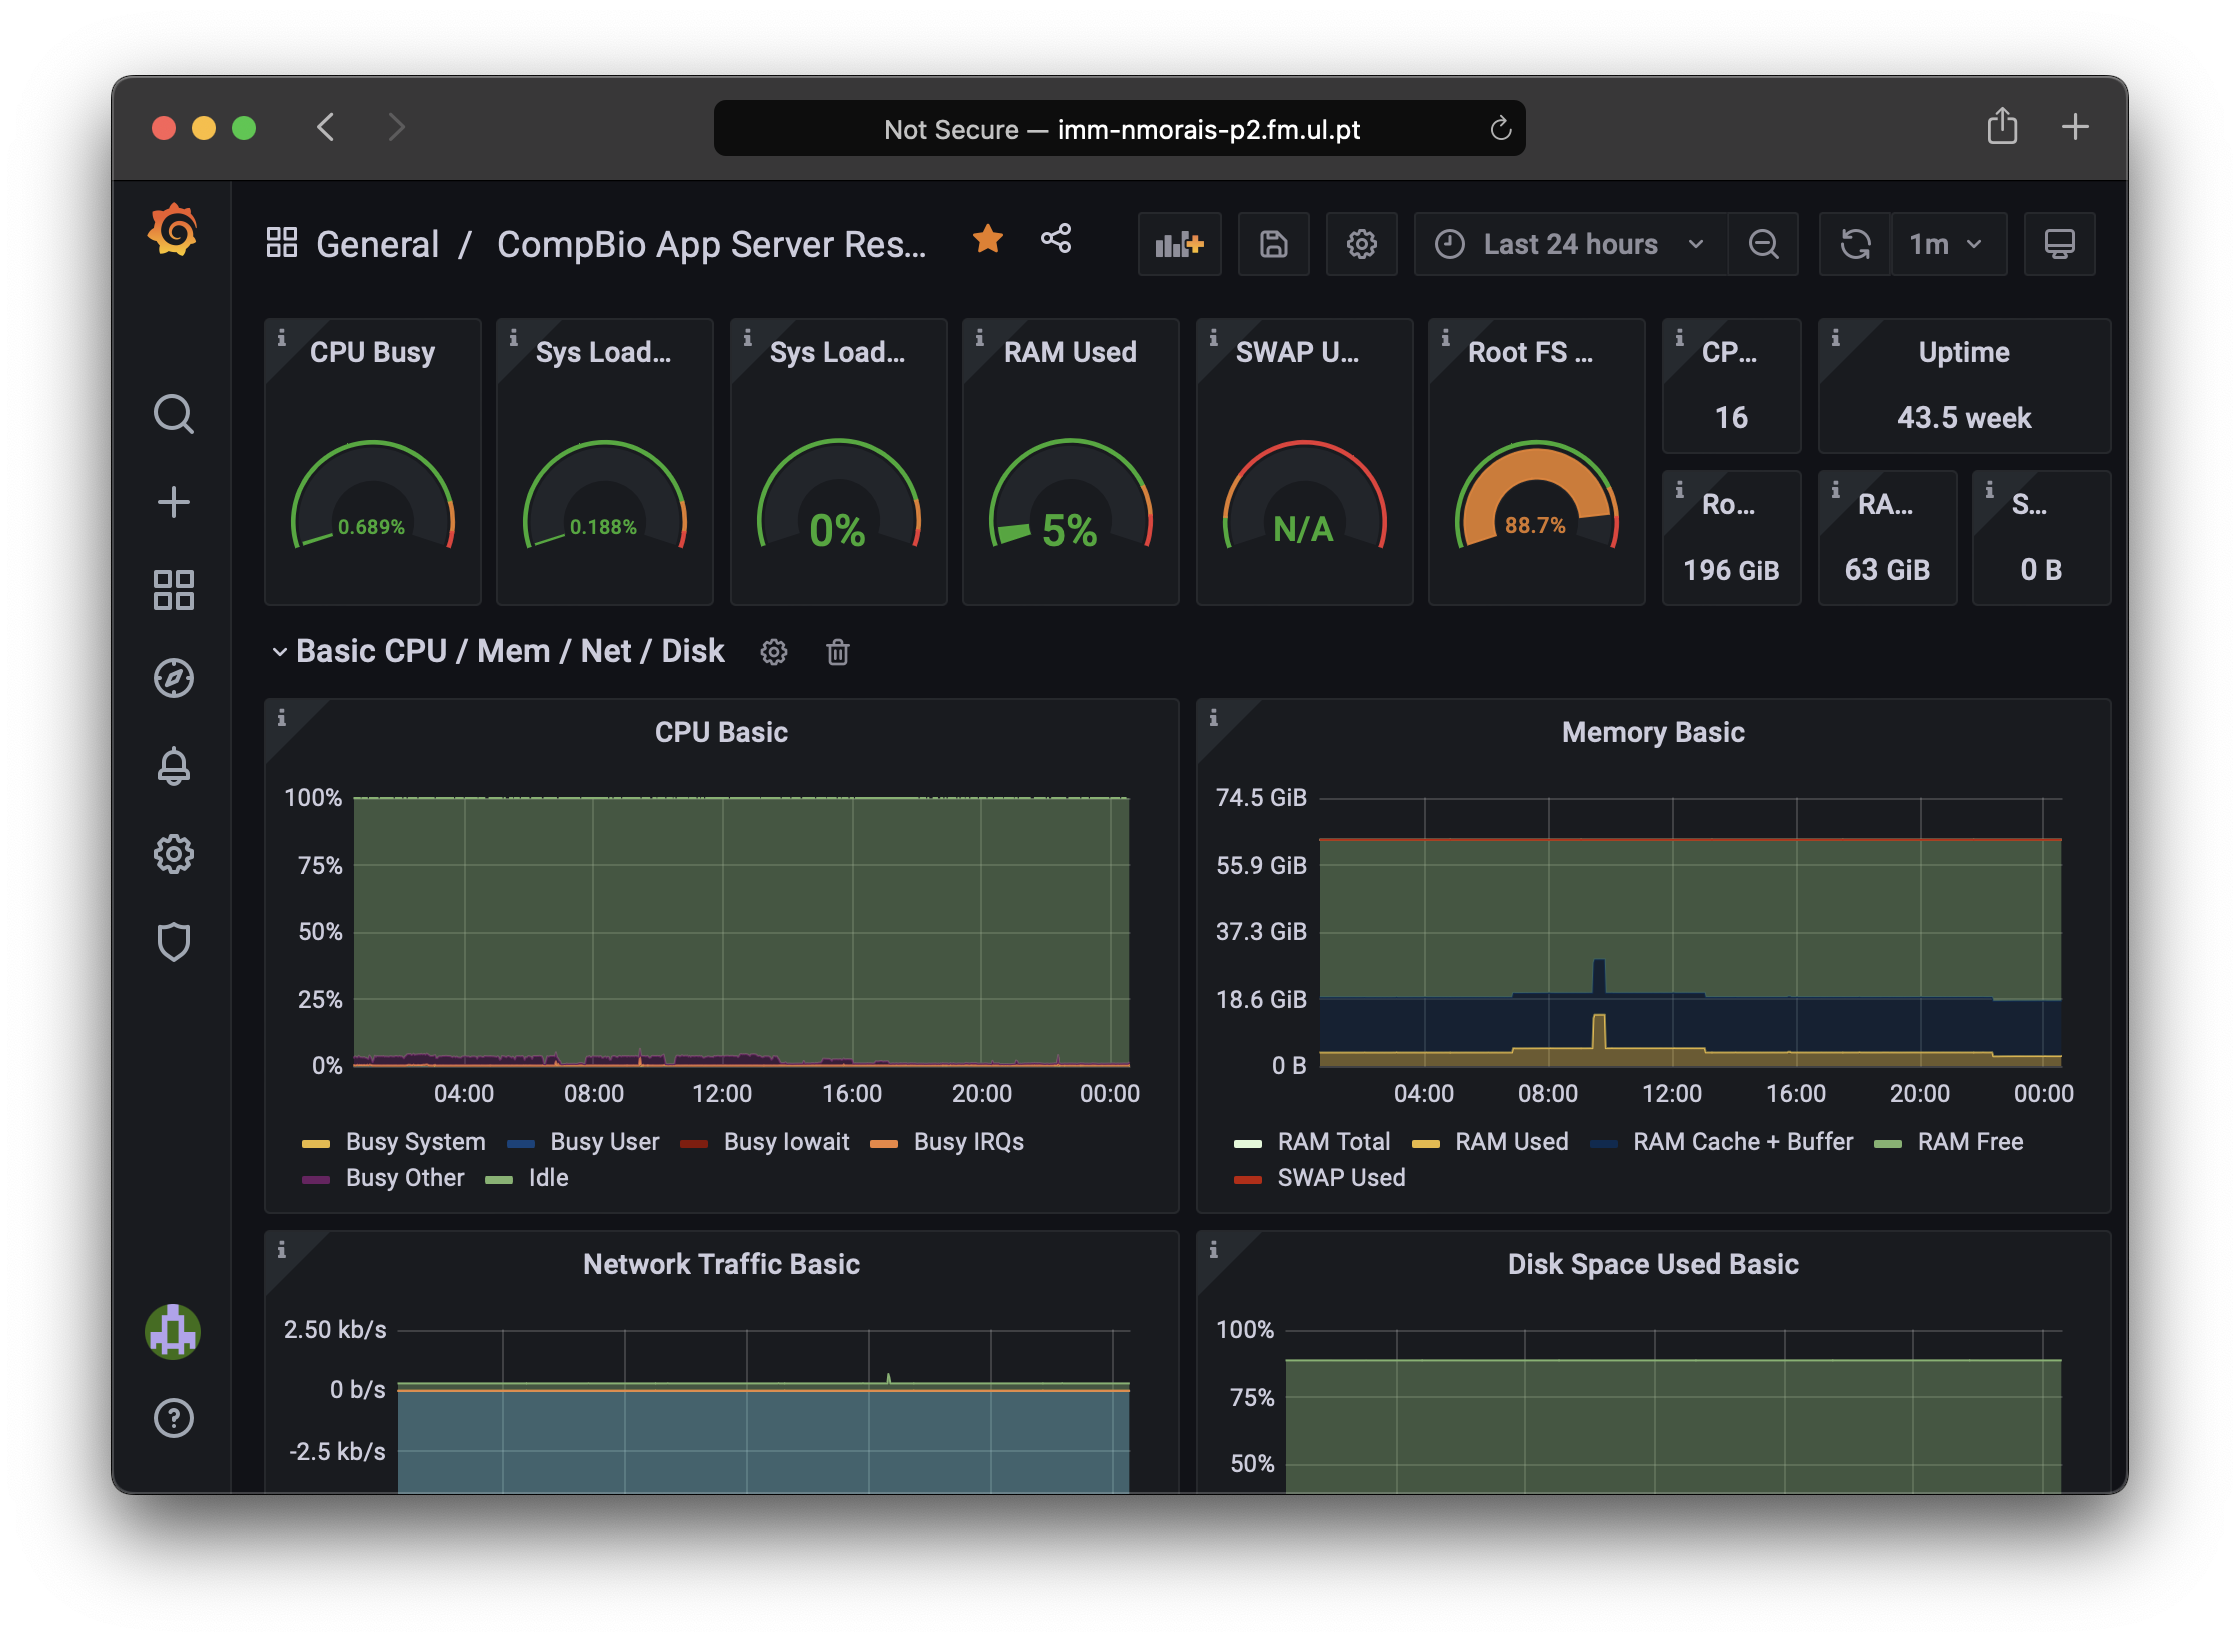
\includegraphics[width=\textwidth]{images/app-server/grafana-system}
		\caption{\footnotesize{\texttt{launchDiffExprLoader}}}
	\end{subfigure}
	\begin{subfigure}[h]{0.3\textwidth}
		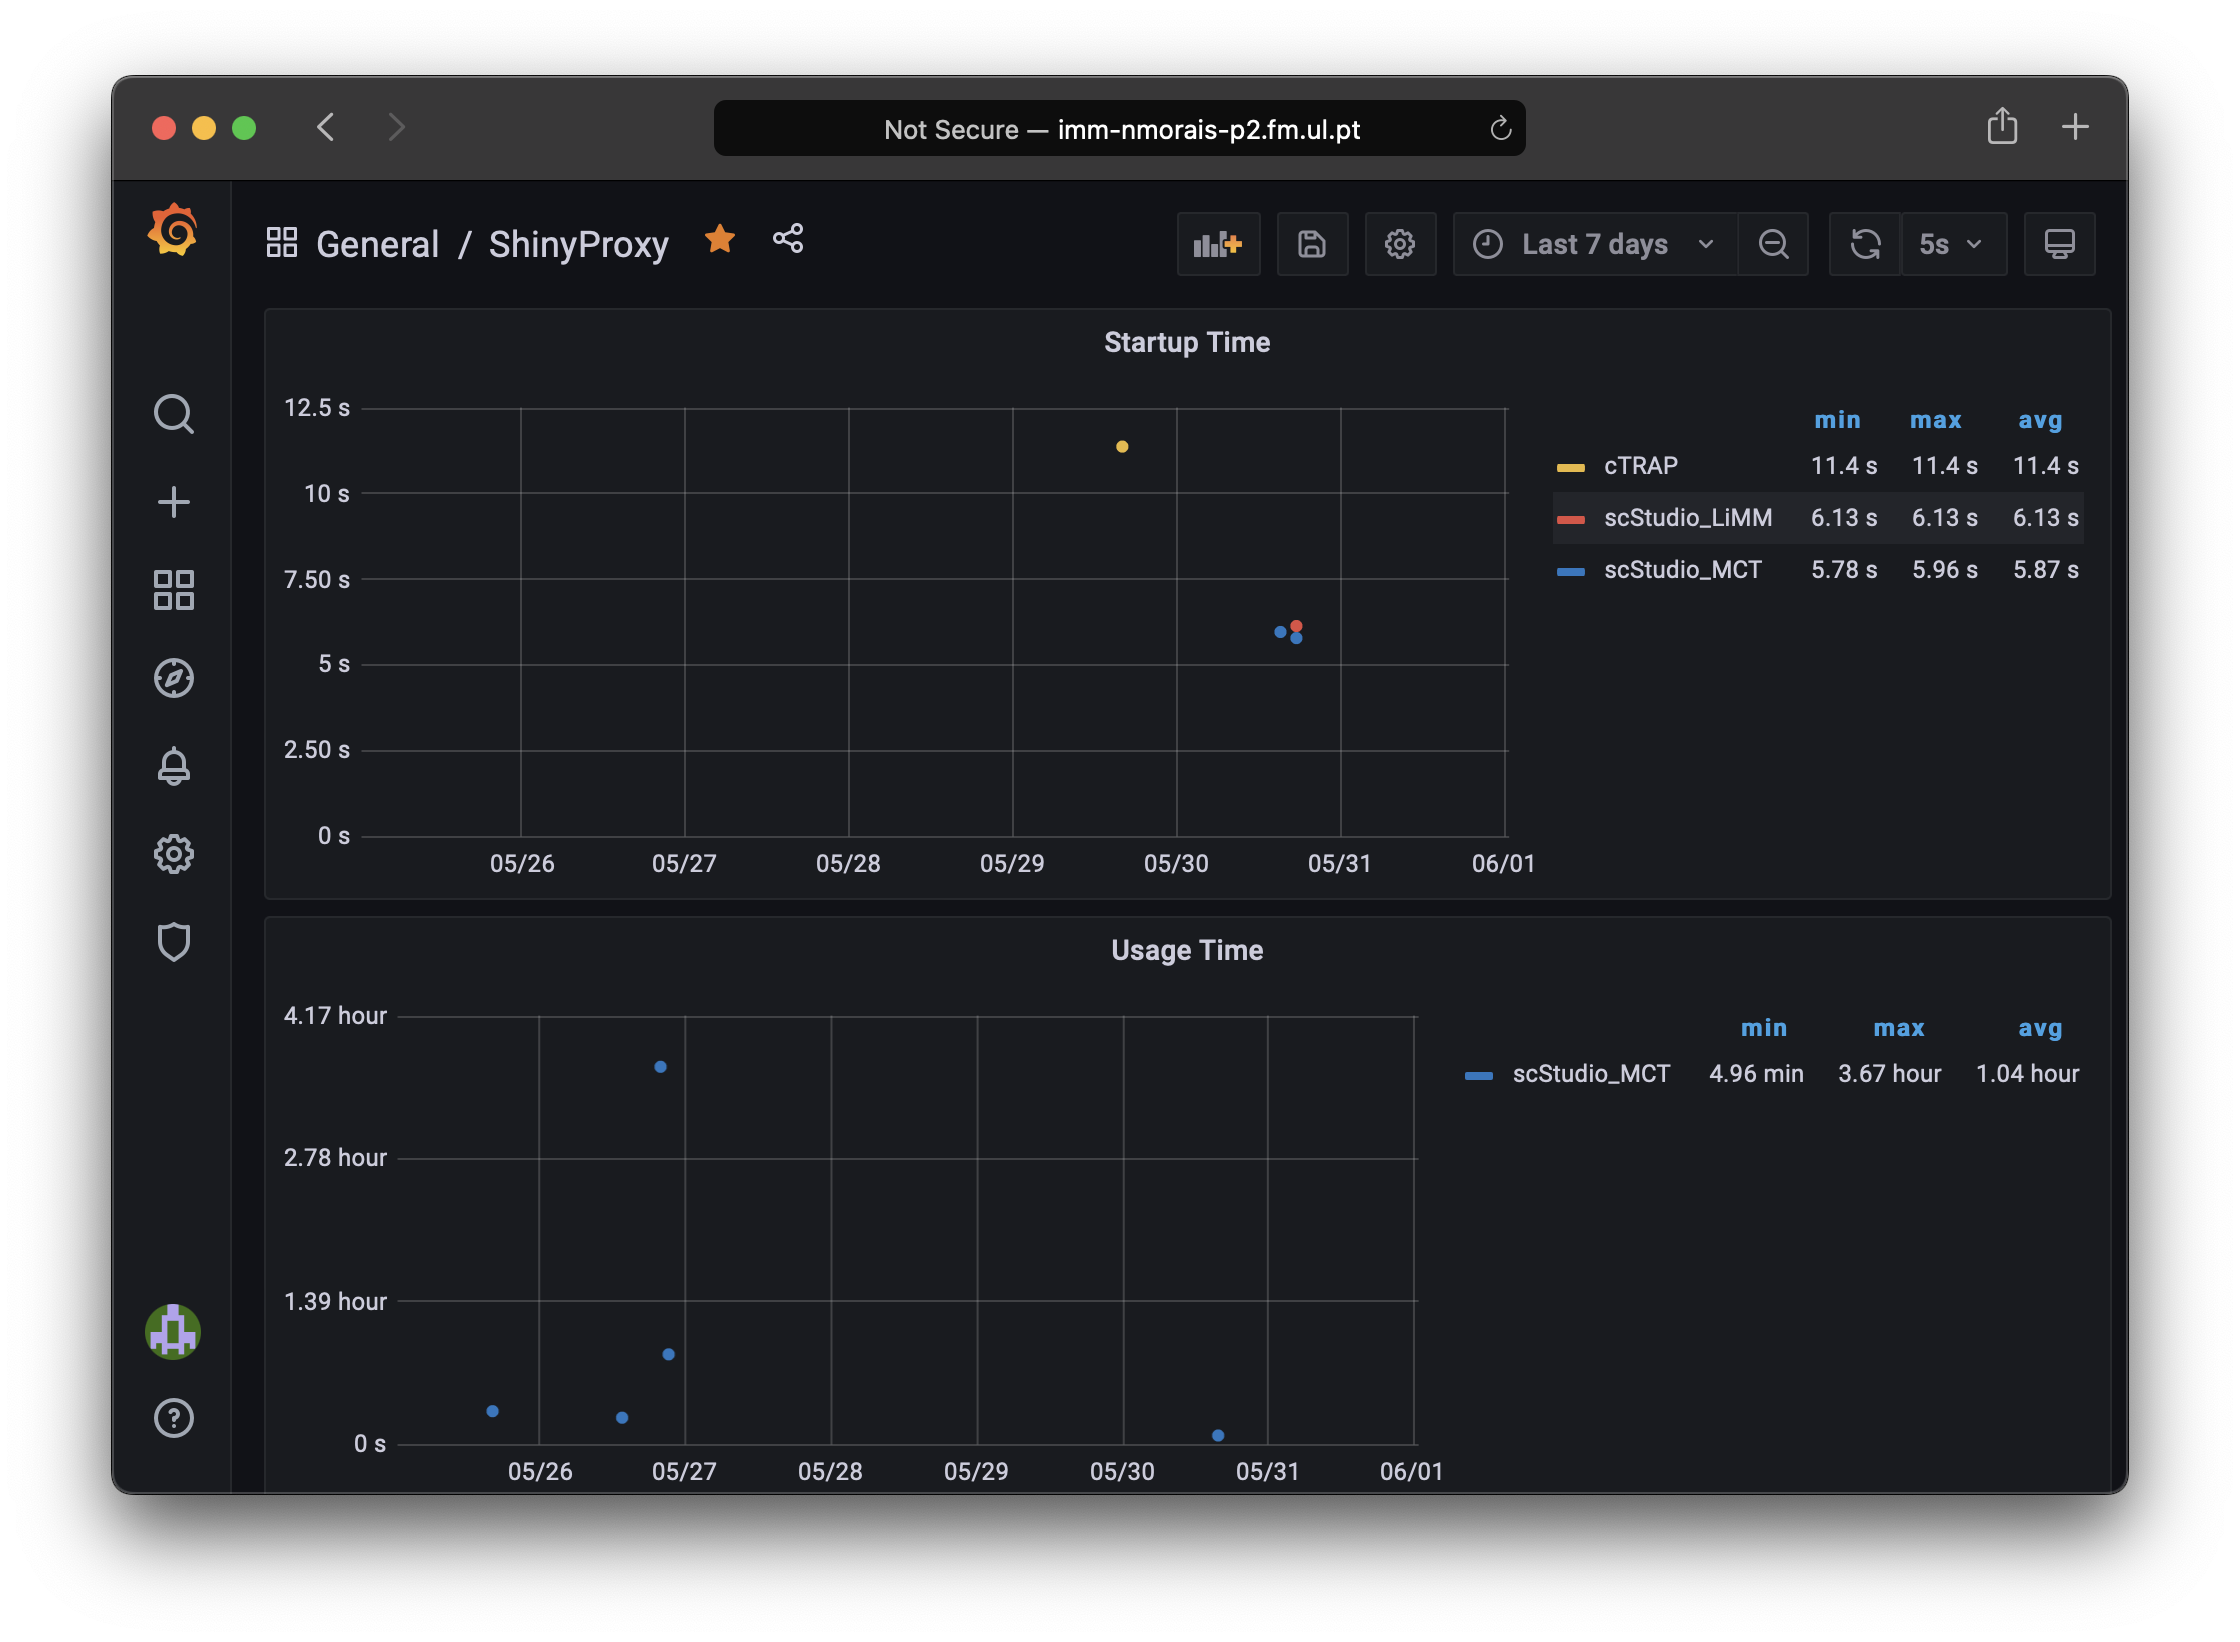
\includegraphics[width=\textwidth]{images/app-server/grafana-shinyproxy}
		\caption{\footnotesize{\texttt{launchCMapDataLoader}}}
	\end{subfigure}
	\begin{subfigure}[h]{0.3\textwidth}
		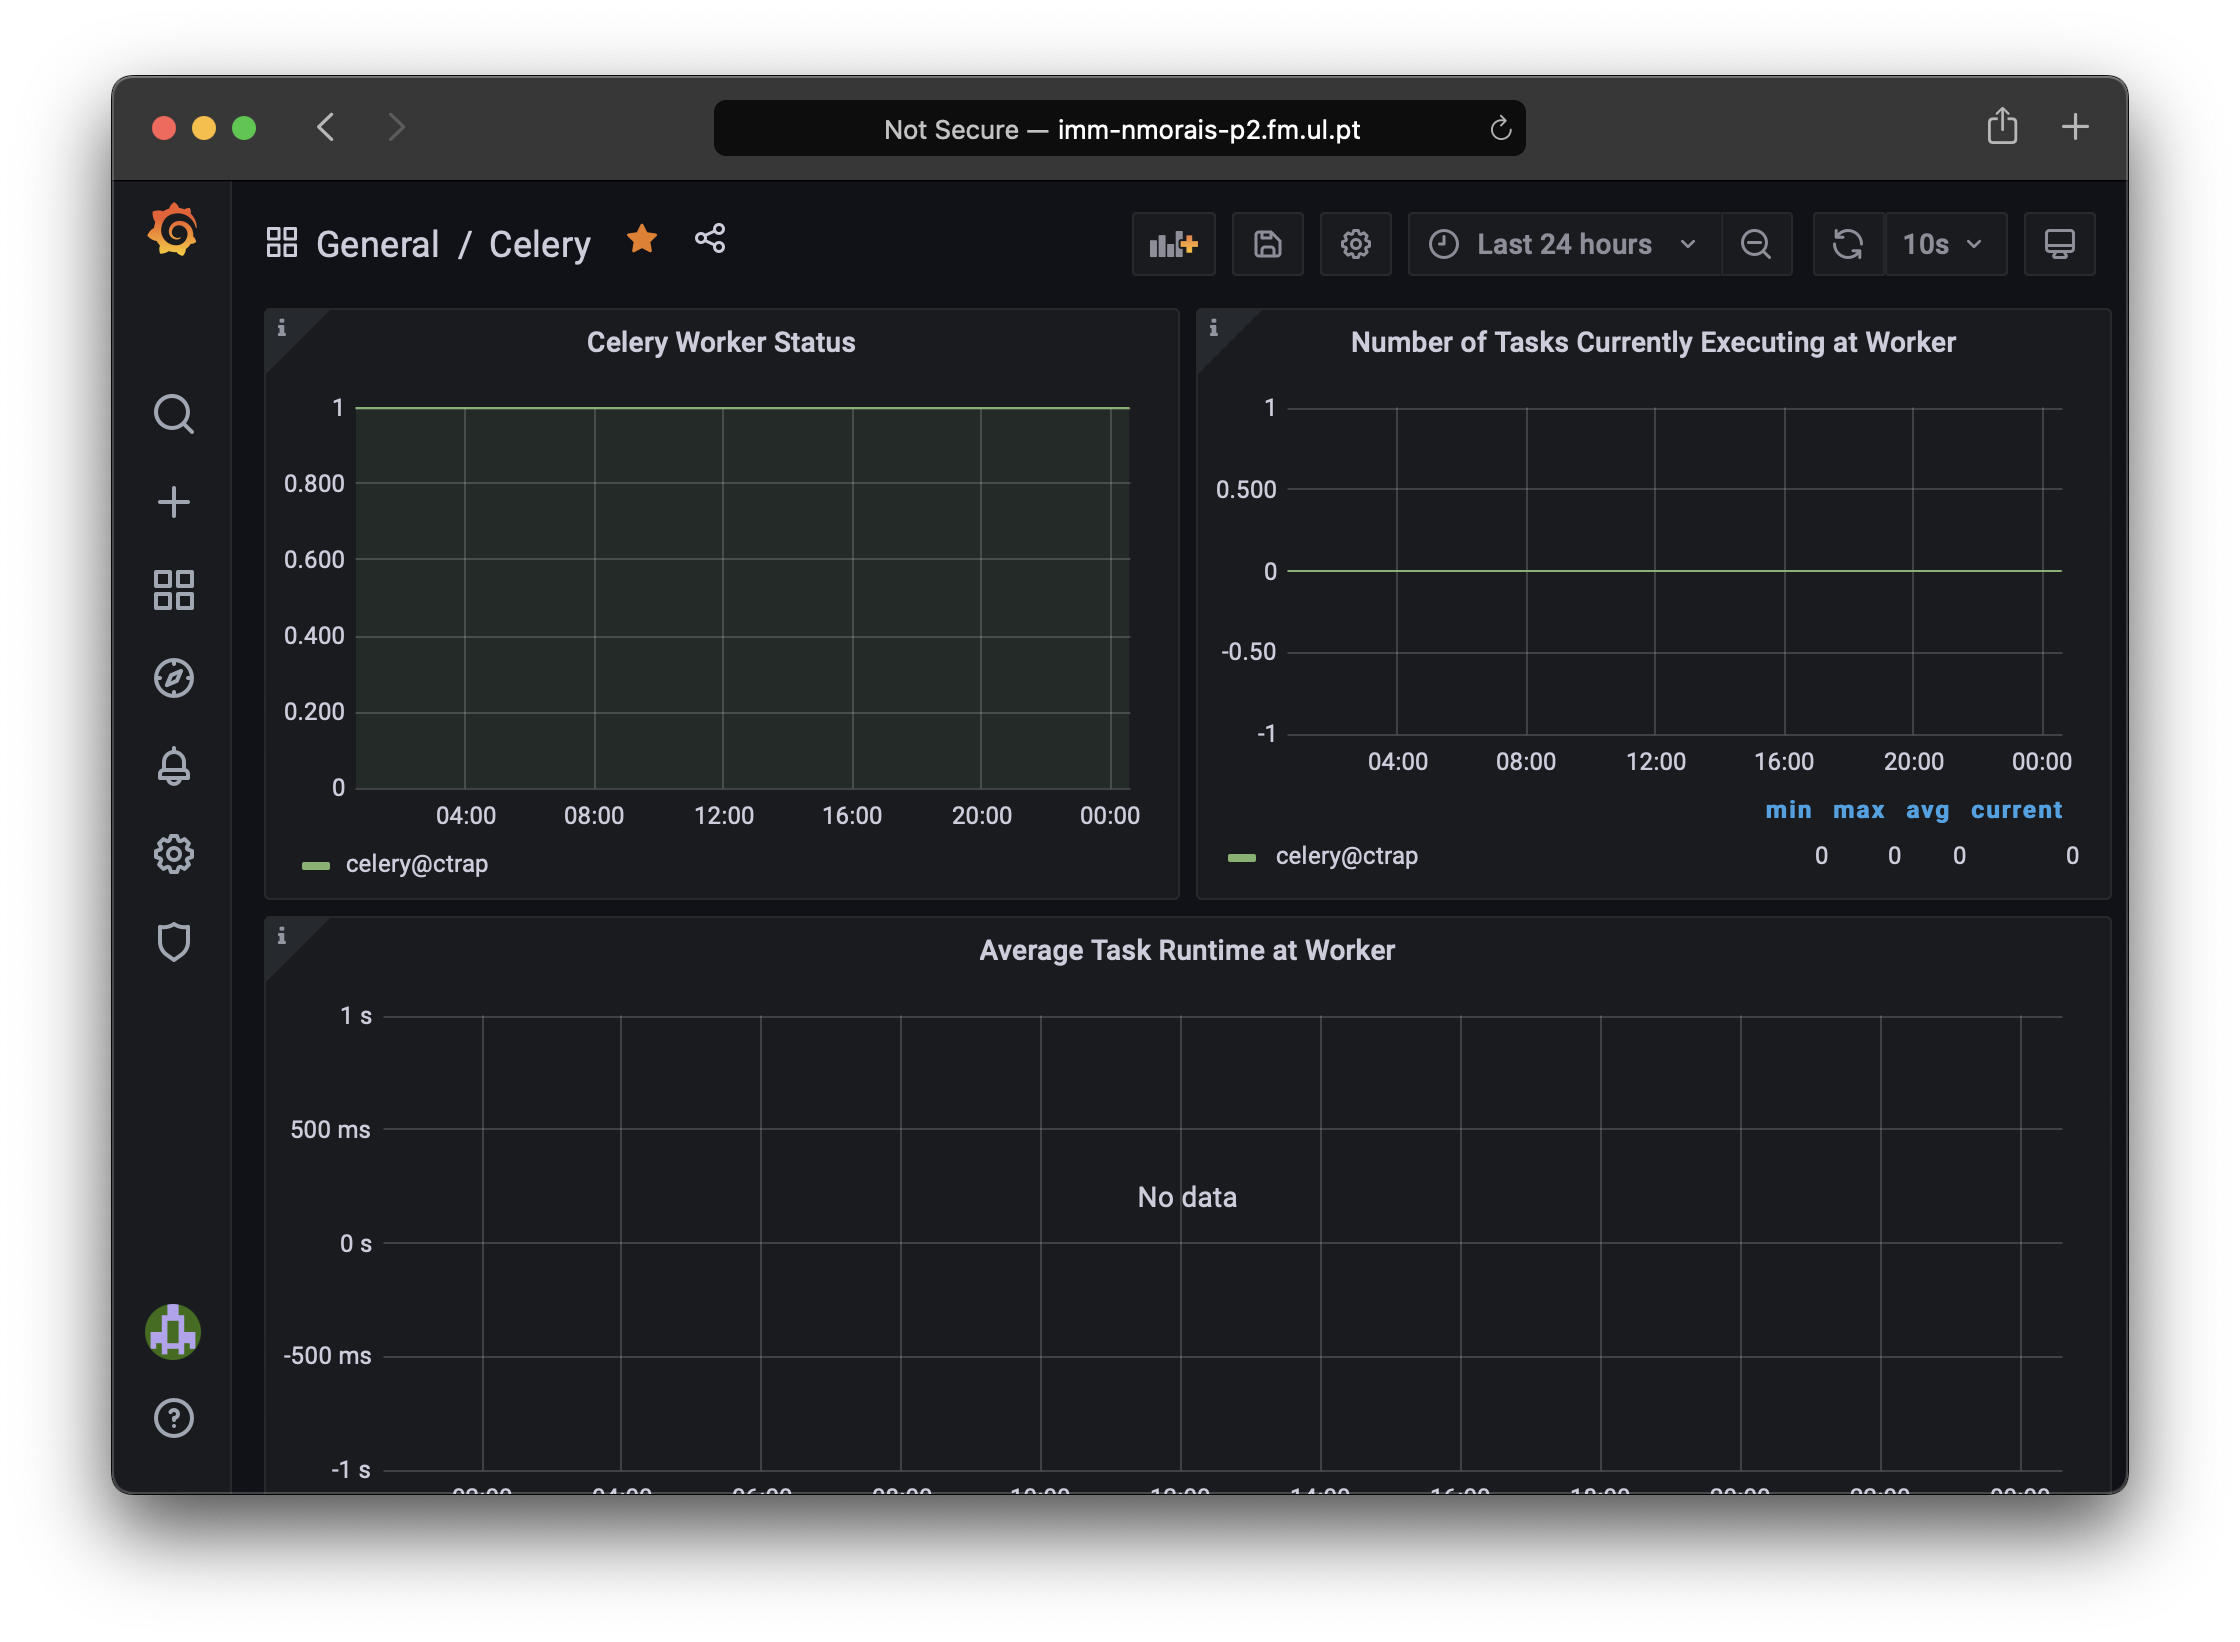
\includegraphics[width=\textwidth]{images/app-server/grafana-celery}
		\caption{\footnotesize{\texttt{launchMetadataViewer}}}
	\end{subfigure}
	\begin{subfigure}[h]{0.45\textwidth}
		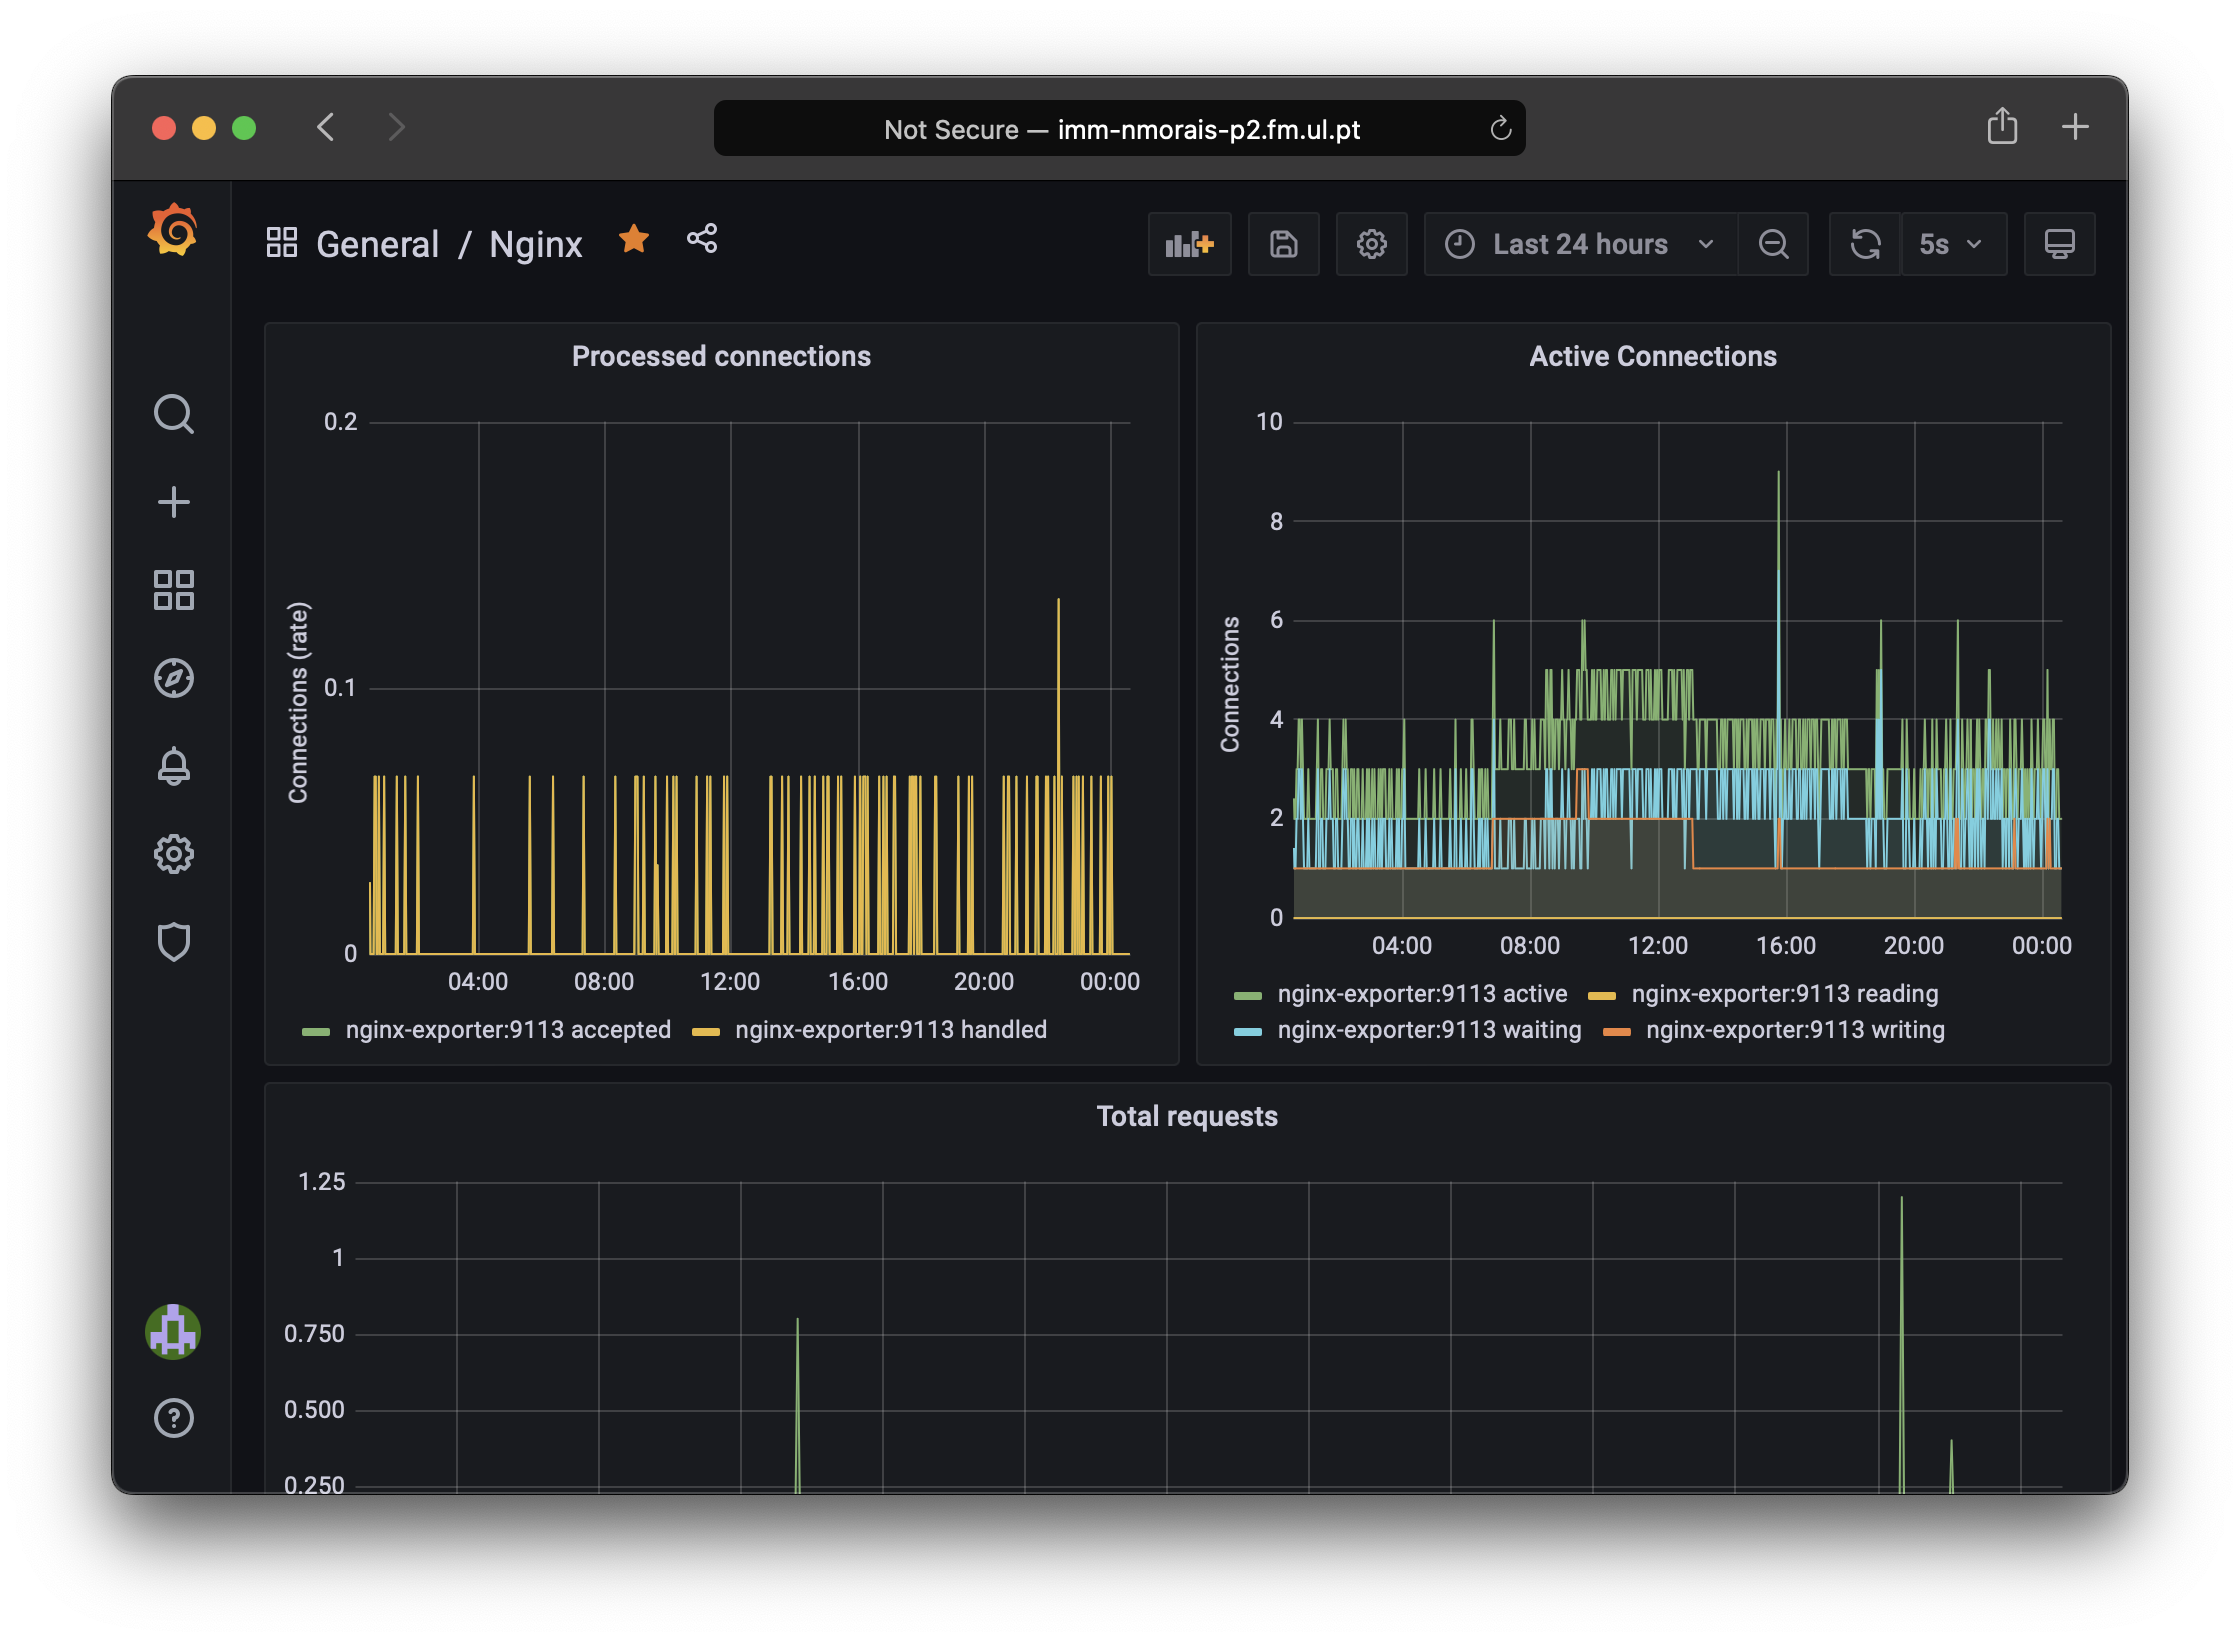
\includegraphics[width=\textwidth]{images/app-server/grafana-nginx}
		\caption{\footnotesize{\texttt{launchResultPlotter}}}
	\end{subfigure}
	\begin{subfigure}[h]{0.45\textwidth}
		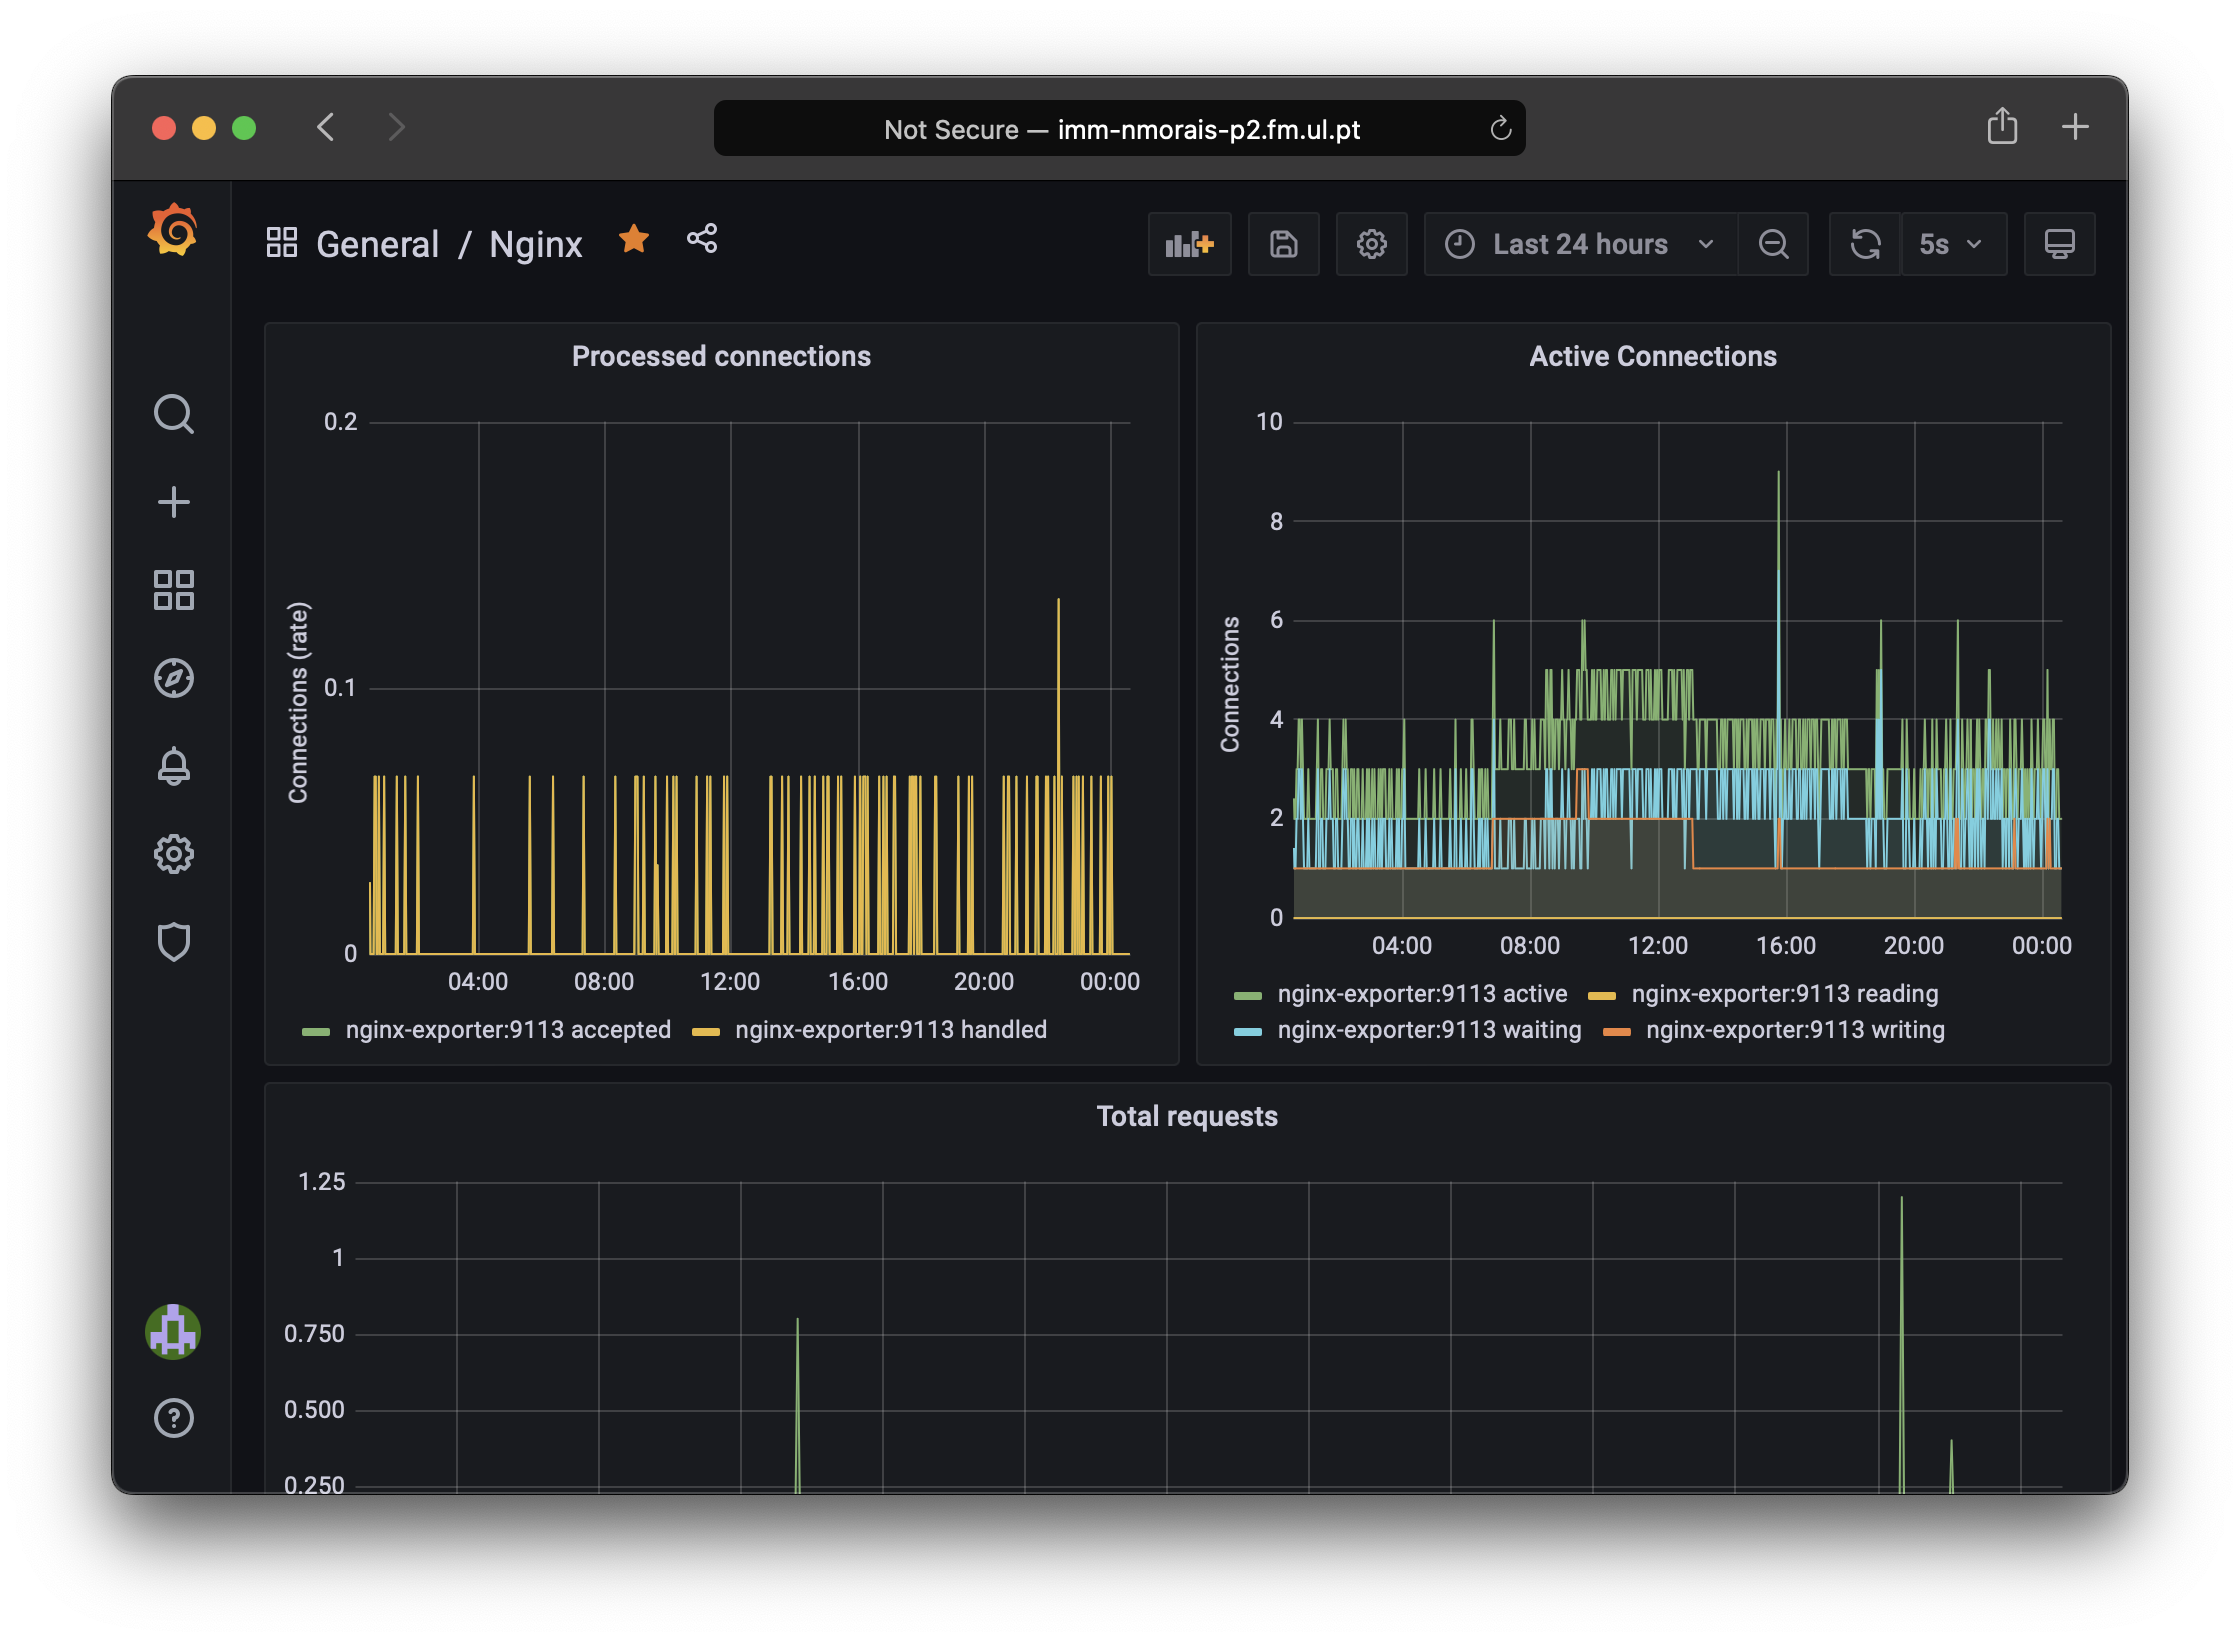
\includegraphics[width=\textwidth]{images/app-server/grafana-nginx}
		\caption{\footnotesize{\texttt{launchDrugSetEnrichmentAnalyser}}}
	\end{subfigure}
	\caption[cTRAP graphical interface functions]{\textbf{cTRAP graphical interface functions}.}
	\label{fig:ctrap-ui-functions}
\end{figure}

Like usual R functions, these graphical interfaces functions accept input arguments and may return output, allowing to intertwine them with R code (\shortref{lst:cTRAP-graphical}). Therefore, users can interactively prepare and explore data before running long-running tasks in the command-line, avoiding the need to have Shiny working while the tasks run (which may also slow down those tasks) and allowing to parallelise them.

\begin{lstlisting}[caption=Calling cTRAP's graphical interface functions in an R script.,label={lst:cTRAP-graphical},language=R,morekeywords={include, launchDiffExprLoader},keywordstyle=\bfseries]
# Launch differential expression loading interface to select knockdown
# data from ENCODE (pre-filtered for HepG2 cell line and EIF4G1 gene)
diffExpr <- launchDiffExprLoader(cellLine="HepG2", gene="EIF4G1")

# After filter selection, launchDiffExprLoader() does the following:
# 1. Download ENCODE's HepG2 data for EIF4G1 knockdown and controls
# 2. Perform DGE between EIF4G1 knockdown vs. control
# 3. Return resulting t-statistics by gene

# Load CMap knockdown data in HepG2
cmapKD <- launchCMapDataLoader(
    cellLine="HepG2",
    perturbationType="Consensus signature from shRNAs targeting the same gene")
# Load CMap compound data in HepG2
cmapCompounds <- launchCMapDataLoader(cellLine="HepG2",
                                      perturbationType="Compound")
# Load all CMap data in HepG2
cmapPerts <- launchCMapDataLoader(cellLine="HepG2")

# View metadata of all resulting CMap data objects
launchMetadataViewer(cmapKD, cmapCompounds, cmapPerts)

# Rank similar perturbations -----------------------------------------
compareKD        <- rankSimilarPerturbations(diffExpr, cmapKD)
compareCompounds <- rankSimilarPerturbations(diffExpr, cmapCompounds)
comparePerts     <- rankSimilarPerturbations(diffExpr, cmapPerts)

launchResultPlotter(compareCompounds, compareKD, comparePerts)

# Predict targeting drugs --------------------------------------------
listExpressionDrugSensitivityAssociation()
assocMatrix <- listExpressionDrugSensitivityAssociation()[[1]]
assoc       <- loadExpressionDrugSensitivityAssociation(assocMatrix)
predicted   <- predictTargetingDrugs(diffExpr, assoc)
launchResultPlotter(predicted)

# Plot targeting drugs vs similar perturbations ----------------------
launchResultPlotter(predicted, compareCompounds)

# Analyse drug set enrichment ----------------------------------------
descriptors <- loadDrugDescriptors("NCI60", "3D")
drugSets    <- prepareDrugSets(descriptors)

launchDrugSetEnrichmentAnalyser(drugSets, compareCompounds)
launchDrugSetEnrichmentAnalyser(drugSets, predicted)
\end{lstlisting}

cTRAP also provides a global visual interface that encompasses all graphical interface modules into one web app by running function \texttt{cTRAP()}, the basis for its online version\footnote{More information in \fullref{chap:app-server}.}. However, by having a single interface, an entire cTRAP session needs to be live and consuming useful resources during the long-running cTRAP analyses, which does not properly scale in a web server with multiple users using heavy memory resources simultaneously. To avoid this, long-running tasks can be optionally managed via job queues running in the background. But this also means that the system must allow for users to get their results back once they finish calculating. And thus the idea of user sessions was born.

\subsubsection{User sessions}
\label{sec:ctrap-web}

\begin{wrapfigure}{r}{.4\textwidth}
  \vspace{-2\intextsep}
  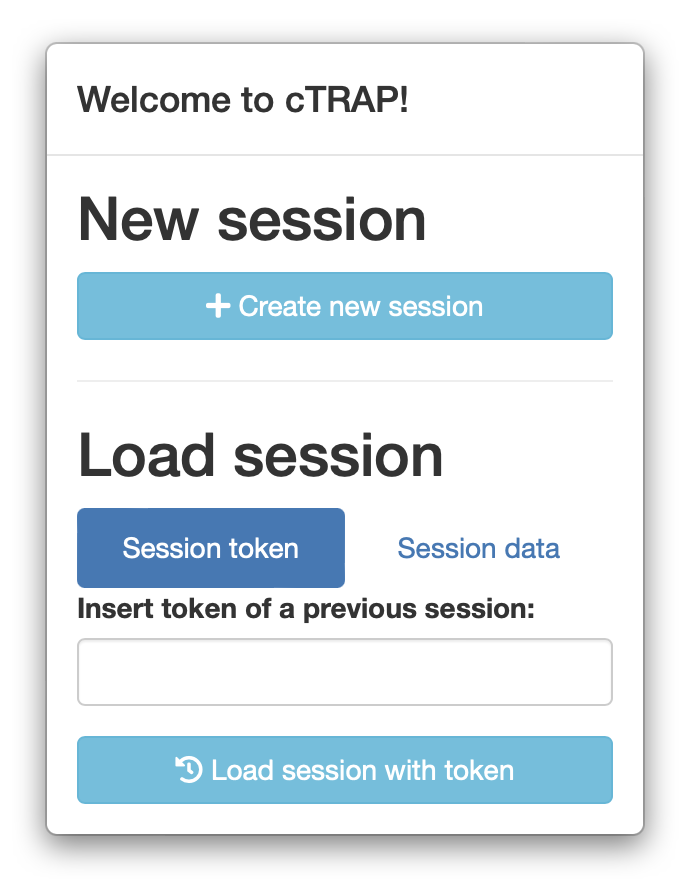
\includegraphics[width=\linewidth]{images/ctrap/welcome}
  \caption[Welcome screen modal]{\textbf{Welcome modal.}}
  \vspace{-1\intextsep}
  \label{fig:ctrap-welcome}
\end{wrapfigure}

Session data are saved in folders named after a random alphanumeric string (token) that uniquely identifies each session and can be downloaded as RDS files. Given that the downloaded file is a list of all datasets from the user session, users can load these RDS files in any R session and in local instances of cTRAP. Downloading user sessions is encouraged because cTRAP session folders are removed from our server if not accessed in the last 30 days based on the access timestamp\footnote{In Linux, the access timestamp (\texttt{atime} attribute) for a directory indicates the last time a file within was read/written or its contents were listed.}.

cTRAP visitors are greeted with a welcome screen that allows them to create a new session or restore previous ones (\autoref{fig:ctrap-welcome}), a dialog that can be opened at any time from the session menu.

% TODO: mention other files in common across cTRAP?
When creating a new session, a unique a token is created. As soon as session-specific data is loaded, a new folder is created in the working directory and named after the session token (\autoref{fig:user-session}). Any updates to the session data are automatically saved to the session folder. To avoid downloading commonly-used files (e.g. the 21GB CMap perturbations z-scores file), an appropriate folder stores data shared across sessions, thus avoiding downloading, storing and processing redundant data.

When restoring a session via a token, cTRAP loads the contents of the folder named after the token located in cTRAP working directory or warns the user if no such folder exists (\autoref{fig:user-session}). In case the user uploads a RDS file of a previous session, cTRAP will load its contents in a new session (\autoref{fig:user-session}).

\begin{figure}[!ht]
  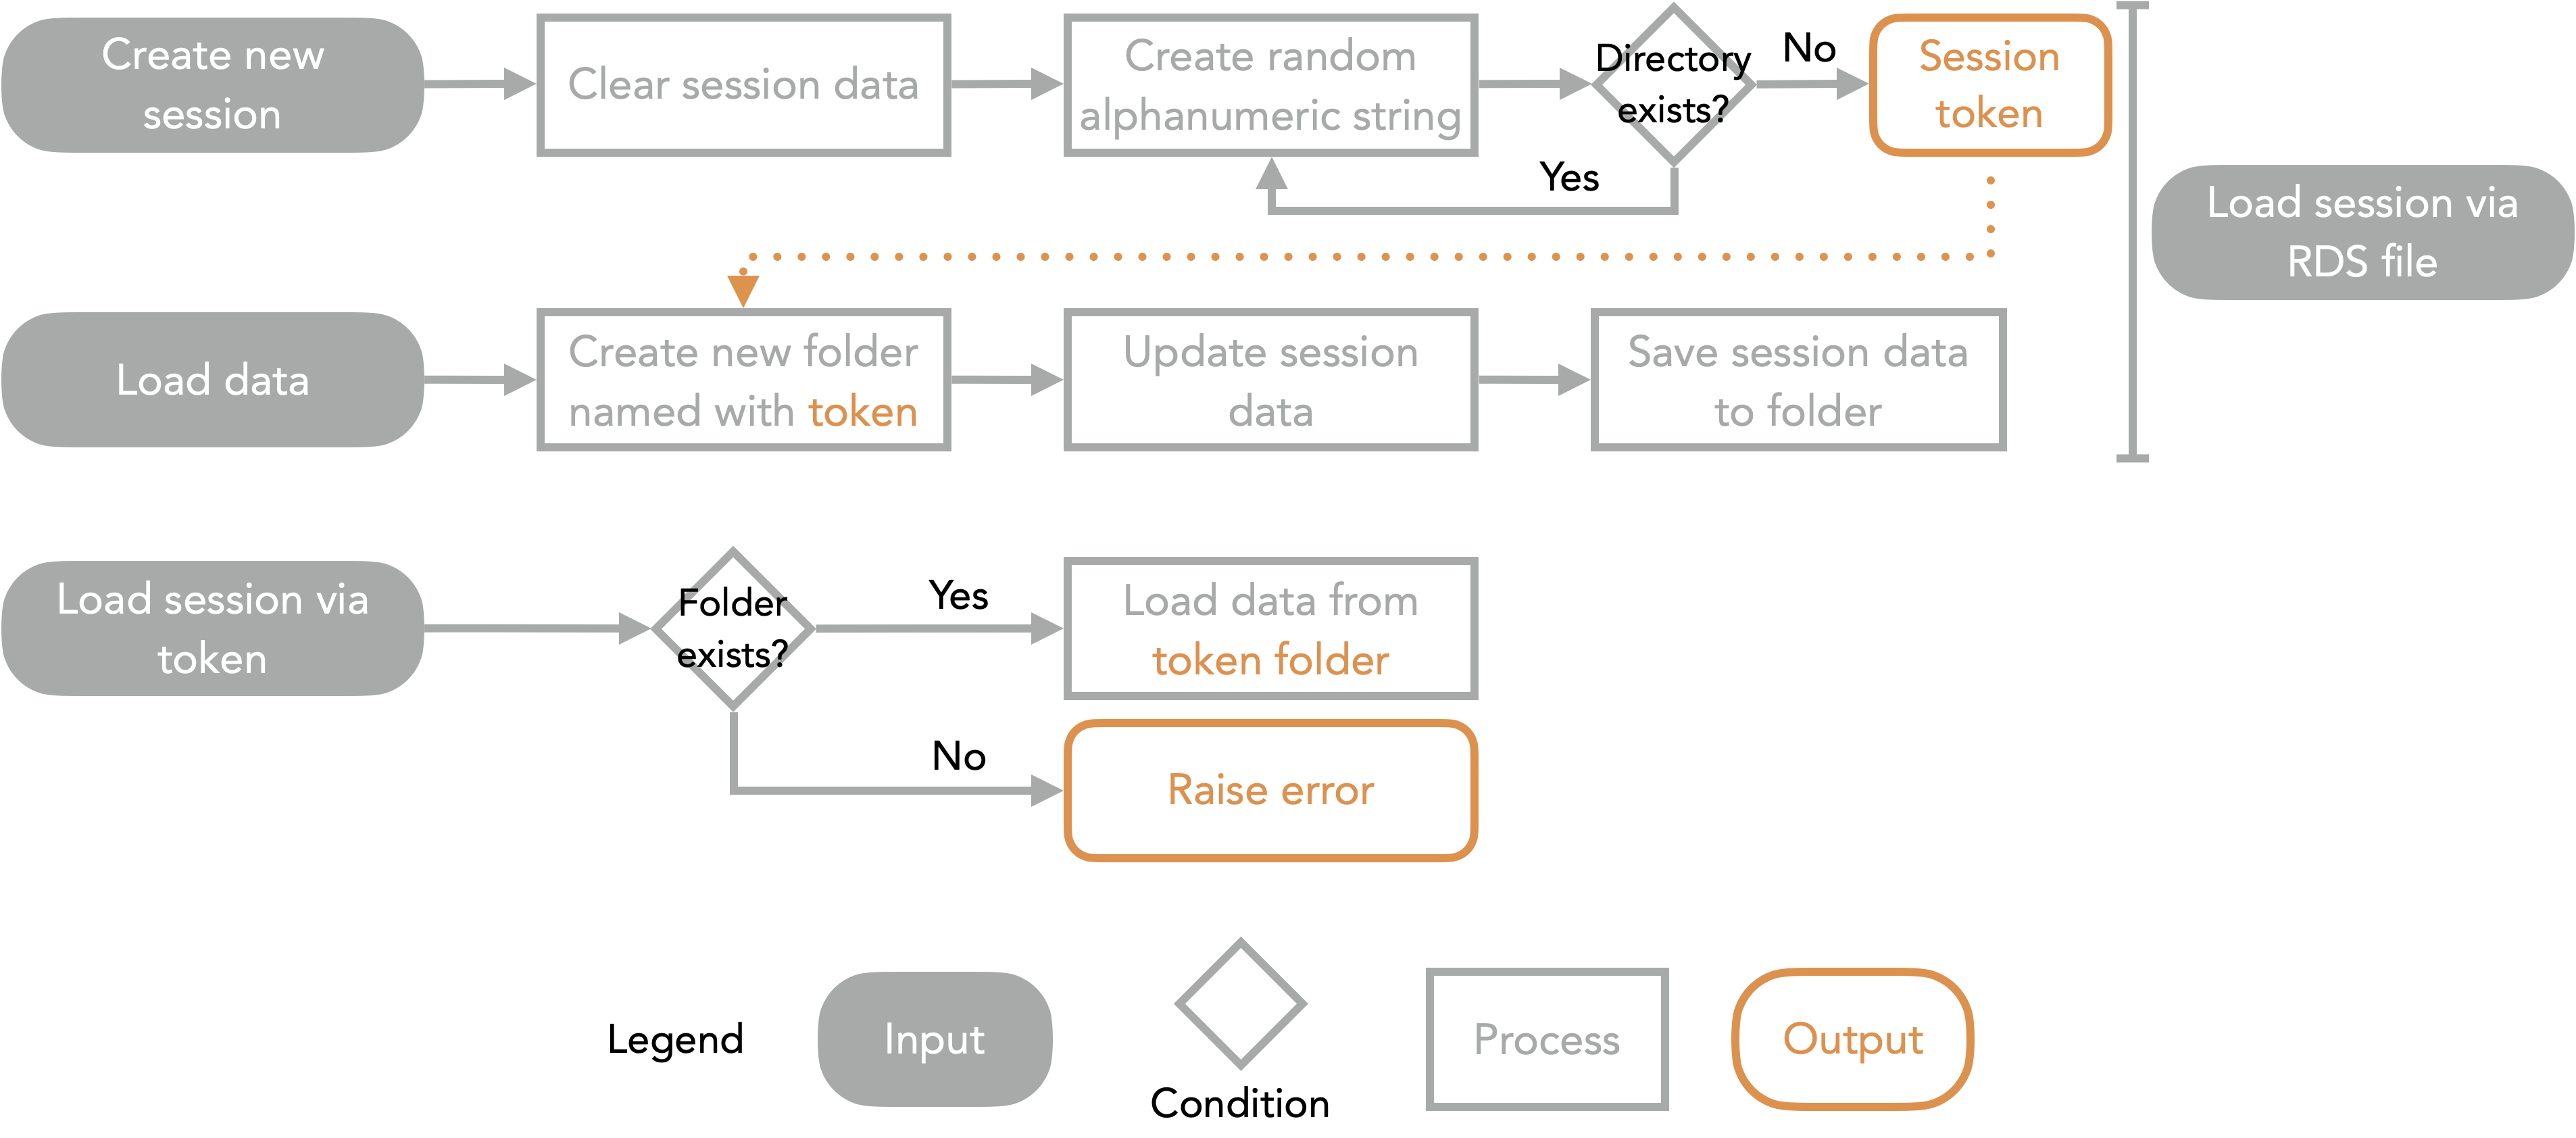
\includegraphics[width=\textwidth]{images/ctrap/user-session}
  \centering
  \caption[User session workflow]{\textbf{User session workflow.} cTRAP allows to create new sessions or load a previous one via a given token or RDS file. When loading session via a RDS file, a new cTRAP session is created before loading the data from RDS file. Sessions can also be loaded using a token if any folder with such token exists in cTRAP's working directory.}
  \label{fig:user-session}
\end{figure}

\subsubsection{Background tasks}
\label{subsec:background-tasks}

When running a Shiny app, the user has to wait for the long-running tasks to finish before the app starts responding to user's commands again. Critically, if cTRAP is shut down, all running processes will stop.

This can be solved by using the R packages \texttt{promises}/\texttt{future} or by manually running another R process in the background. However, these solutions require the Shiny app to be active during the whole process, which can be especially egregious if the R session is consuming many computing resources, disallowing other apps or users to take advantage of those resources until the whole session is terminated.

What are the best options to run large tasks in the background? In Lobo, iMM's computing cluster, we use a job scheduler for that function: SLURM. However, SLURM is too complex to install -- I was not able to create a working prototype of SLURM for a single machine using Docker or otherwise. Anyway, we can use these light-weight alternatives instead:

\begin{itemize}
	\item \textbf{Celery}, a task queue manager written in Python; and
	\item \textbf{Flower}, a monitoring app that provides an HTTP API and graphical interface to manage Celery jobs.
\end{itemize}

Celery requires a \texttt{tasks.py} file with the code of the jobs to run. Given that Celery will run cTRAP functions, cTRAP must be installed alongside Celery. Moreover, as we intend to run R code, one of the Celery tasks is to run R via Python's module \texttt{subprocess} to spawn new processes with the \texttt{Rscript} command (\shortref{lst:tasks.py}).

\begin{lstlisting}[language=python,caption=An example \texttt{tasks.py} file to run R commands or Rscript files via Celery.,label={lst:tasks.py},morekeywords={import},keywordstyle=\bfseries]{tasks.py}
import os, time
from datetime import datetime
from subprocess import run, PIPE

# Celery configuration
from celery import Celery
os.environ.setdefault('C_FORCE_ROOT', 'true')
app = Celery(
    "tasks",
    broker=os.environ.get('CELERY_BROKER_URL', 'redis://redis'),
    backend=os.environ.get('CELERY_RESULT_BACKEND', 'redis://redis'))
app.conf.CELERY_WORKER_SEND_TASK_EVENTS = True

# Runs R command and returns output
#   - Use cat(), e.g. 'cat(2+2)', to capture output as a job result
#   - Errors will result in a task state of FAILURE
def execR(cmd):
    return run(cmd, check=True, stdout=PIPE, text=True).stdout

# Run a given R expression as a Celery job
@app.task
def R(cmd): return execR(["Rscript", "-e", cmd])

# Run a given Rscript file as a Celery job
@app.task
def Rscript(cmd): return execR(["Rscript", cmd])

if __name__ == "__main__": app.start()
\end{lstlisting}

Flower can send jobs to Celery via HTTP methods, facilitating the communication between cTRAP and Celery. To assist using Flower in R, I created the R package \texttt{floweRy} (\alink{github.com/nuno-agostinho/floweRy}) that contains wrapper functions for most of its HTTP API functions. Internally, \texttt{floweRy} calls HTTP methods with \texttt{httr} R package, creating dedicated commands that make it easier than using just plain \texttt{httr}, as briefly demonstrated in Listings \shorterref{lst:httr} and \shorterref{lst:floweRy}.

\noindent\begin{minipage}{.48\textwidth}
\begin{lstlisting}[caption=Job submission with \texttt{httr}.,language=R,label={lst:httr}]{httr}
library(httr)
flower <- function(...) paste0(
    "http://localhost:5555", ...)
# Run R command '3 + 4' in Celery
POST(flower("/api/task/apply/tasks.R")), body="3 + 4", encode="json")
# Get status of all Celery tasks
GET(flower("/api/tasks"))
\end{lstlisting}
\end{minipage}\hfill
\begin{minipage}{.48\textwidth}
\begin{lstlisting}[caption=Job submission with \texttt{floweRy}.,language=R,label={lst:floweRy}]{floweRy}
library(floweRy)
options(flowerURL=
    "http://localhost:5555")
# Run R command '3 + 4' in Celery
taskApply("tasks.R", "3 + 4")


# Get status of all Celery tasks
taskList()
\end{lstlisting}
\end{minipage}

cTRAP currently supports ranking similar CMap perturbation and predicting targeting drugs as background processes by submitting jobs to Celery with the exact R commands to run via the \texttt{Rscript} command \cite{r-core-team:2021wf}. The status of background tasks can be monitored by users in the respective cTRAP's user session (\shortref{fig:job-progress})\footnote{Flower allows to monitor and manage Celery jobs, but its web interface is only accessible in the iMM network (via ethernet cable or VPN). More information in \fullref{sec:background-tasks}.}.

\begin{figure}[!h]
  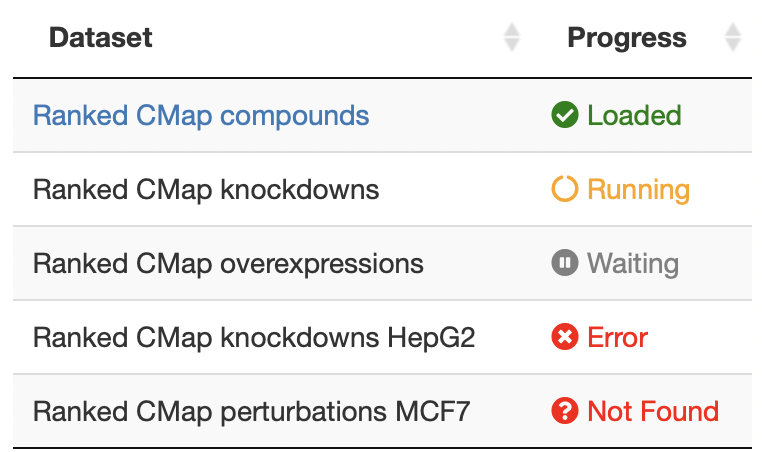
\includegraphics[width=.5\textwidth]{images/ctrap/job-progress}
  \centering
  \caption[Progress of Celery jobs in cTRAP]{\textbf{Progress of Celery jobs in cTRAP.} The job status are updated every 5 seconds. Their status can be: \textcolor{gray}{Waiting} in job queue to start, \textcolor{orange}{Running}, \textcolor{teal}{Loaded}, \textcolor{red}{Error} for unknown failures, and \textcolor{red}{Not Found} if the job results cannot be found (e.g. when re-uploading the same RDS file, the job results were already cleaned-up in the first upload). When jobs are loaded, the dataset name is updated with a link to directly access their results (blue colour).}
  \label{fig:job-progress}
\end{figure}

All Celery jobs are saved as \emph{dummy} objects in cTRAP's user session data, containing the job identifier and metadata from expected results. When the background processes finish, their output is saved into the session folder. If the user is actively using that session in the cTRAP website, the data is automatically loaded -- replacing the previous \emph{dummy} objects -- and the user is informed of such via a notification in cTRAP (\shortref{fig:ctrap-celery}). Otherwise, next time that session is loaded by the user (either via its token or an RDS file), the job for every \emph{dummy} object in the session data is returned if finished.

% TODO: file is removed after its object is loaded: confirm
\begin{figure}[!htb]
  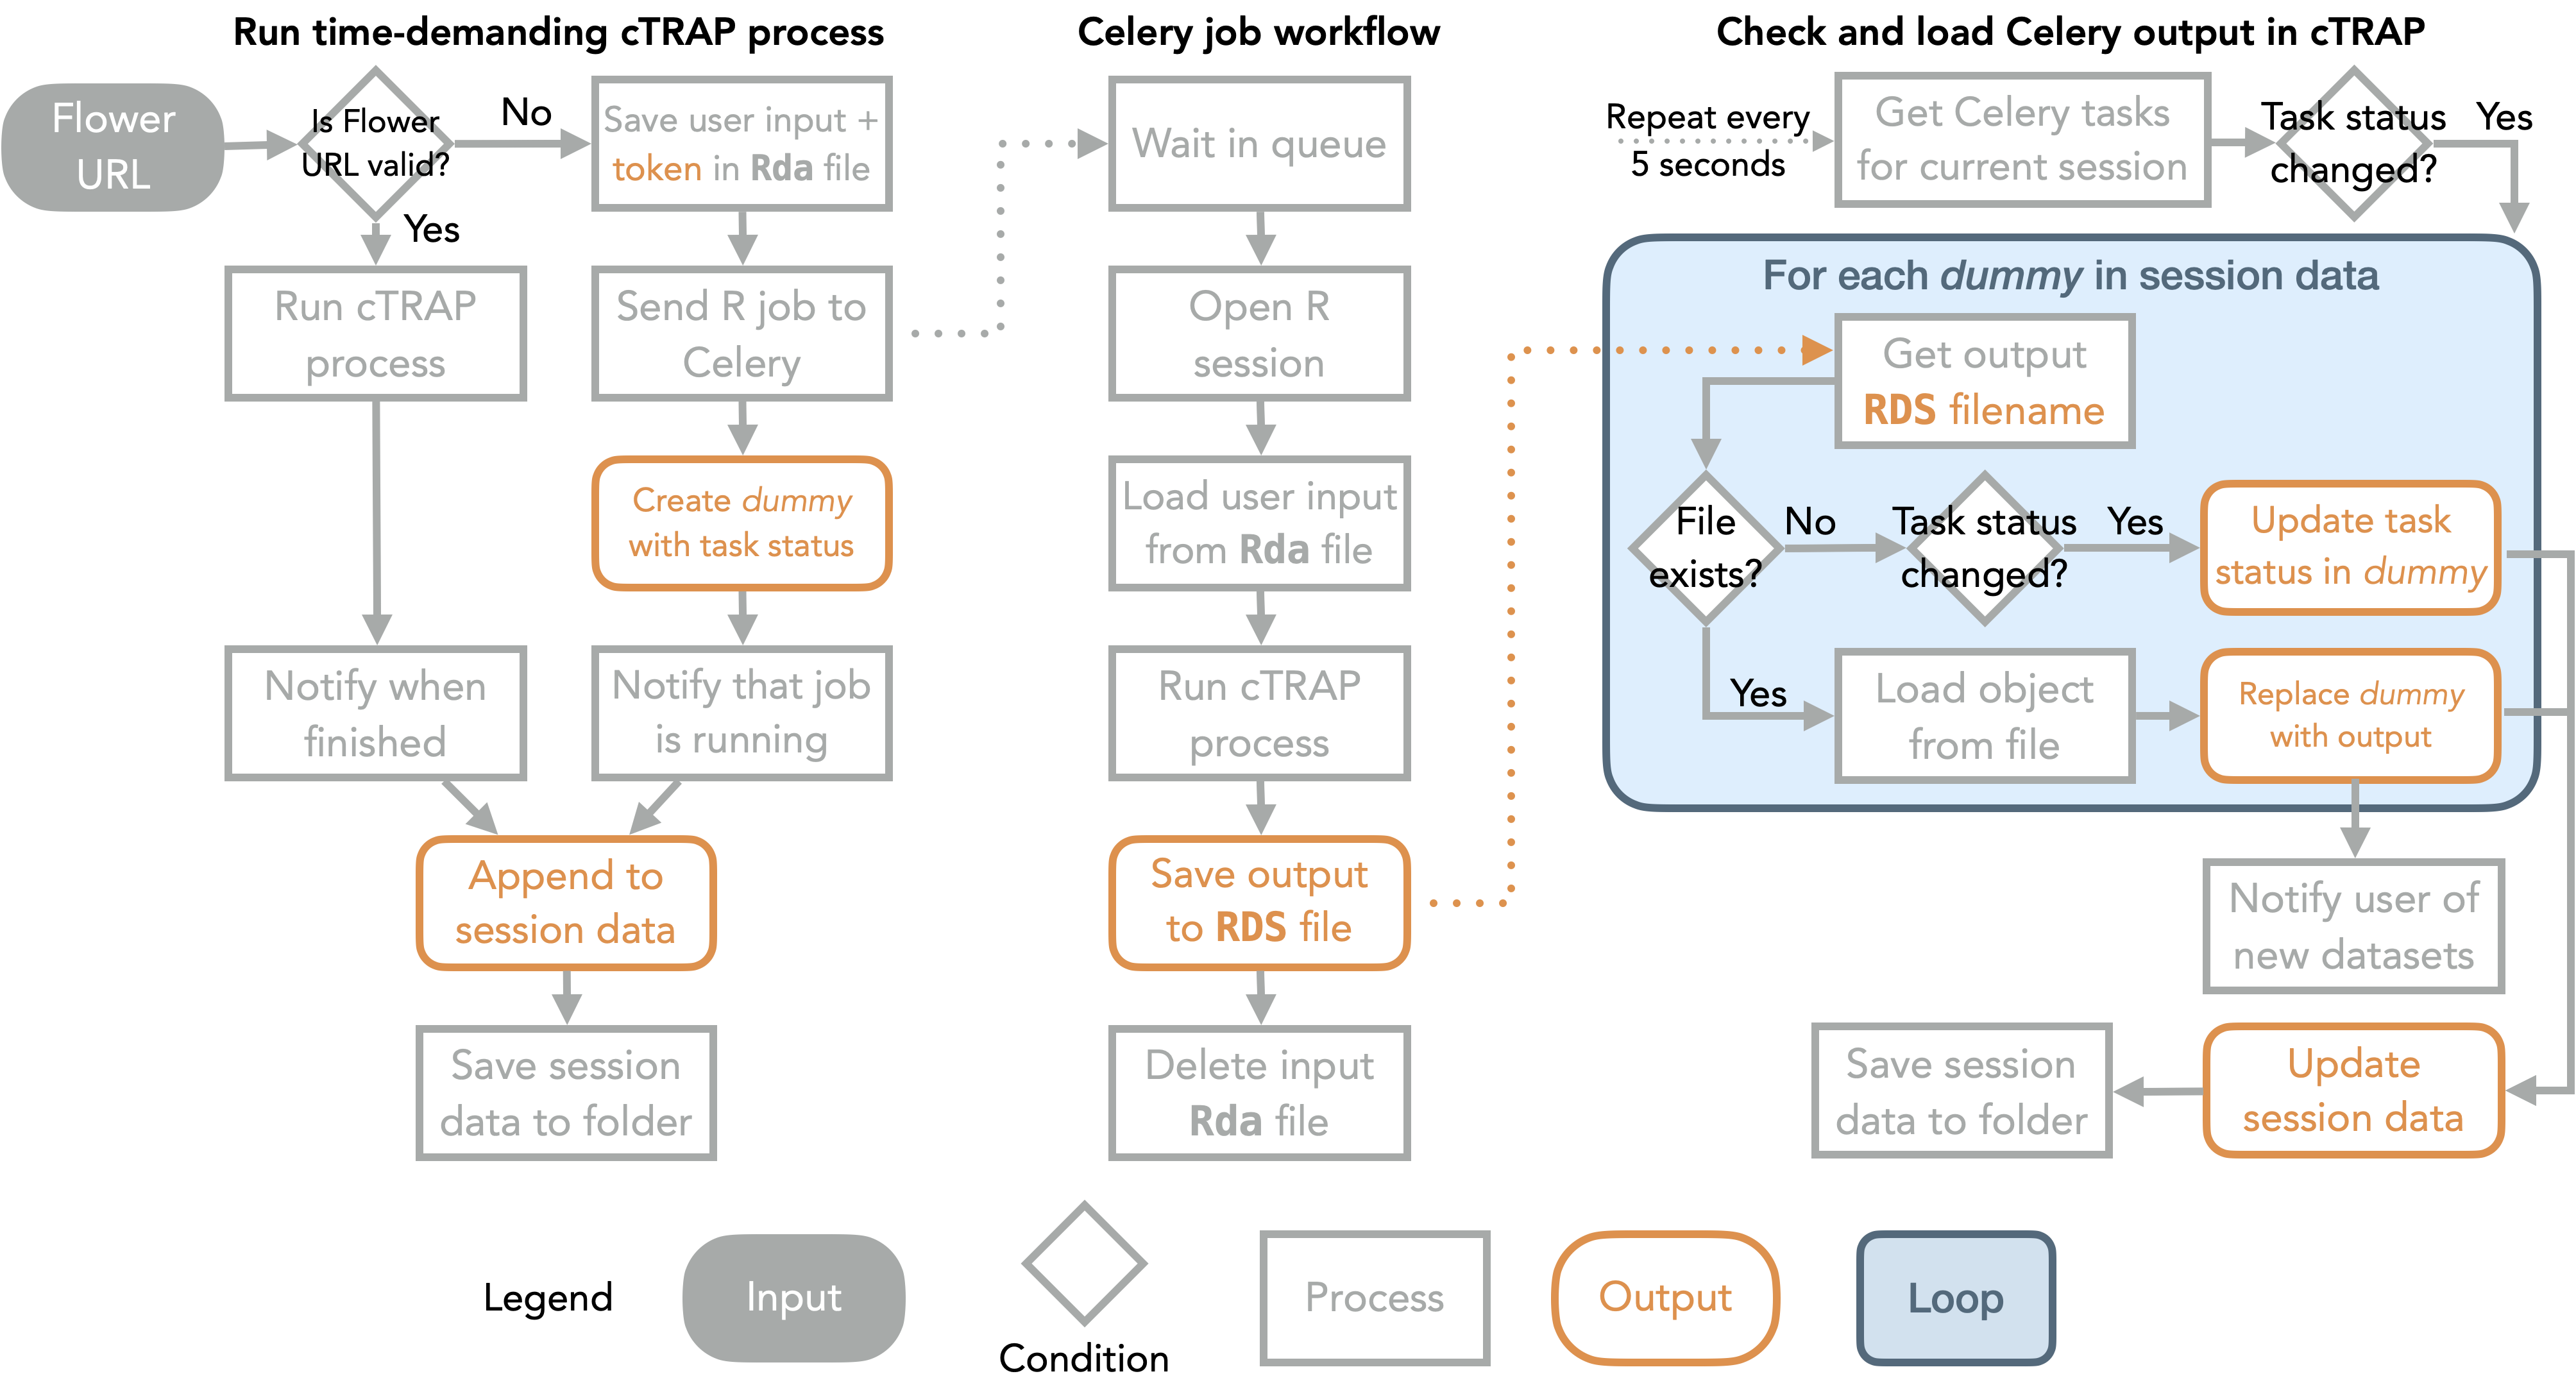
\includegraphics[width=\textwidth]{images/ctrap/celery-job}
  \centering
  \caption[cTRAP process running in Celery]{\textbf{cTRAP process running in Celery.} Time-demanding cTRAP processes can be run in the background using Celery/Flower. While running in Celery, the output of the cTRAP process is saved to the folder associated with the token of the user's session. When that specific session is active, all finished files are automatically loaded as part of the data session and the user is notified.}
  \label{fig:ctrap-celery}
\end{figure}

\section{Conclusion}

% what is your main finding (ANSWER)
% how are your findings with respect to the literature (POSITIONING)
% - RESULT: the actual results
% - CONTEXT: literature search
% - LINK: between my findings and what is known
% - INTERPRETATION: where you pinpoint, suggest, propose...
% what is your main contribution (CONTRIBUTION)
% what are the limitations (LIMITATIONS)
% what are the next steps (ENDING/FUTURE WORK)

CMap is a repository of gene expression signatures for thousands of genetic and pharmacological perturbations that can be explored via a collection of web apps available at \alink{clue.io}, which allows to upload user-provided results to compare against the CMap database. However, their queries are limited to a maximum of 150 up-regulated and 150 down-regulated genes, their results use a non-standard significance score and their apps do not run locally. Also, \alink{clue.io} does not make use of publicly available drug sensitivity data that could help narrow down compounds that selectively target cells.

To overcome such issues, we developed cTRAP to identify causal perturbations from differential expression data, as well as pinpoint compounds that may promote or revert observed differences in gene expression. cTRAP allows to analyse the ordered list of resulting compounds to predict targeting drugs based on publicly available drug sensitivity data from NCI60, GDSC and CTRP. Moreover, cTRAP allows to perform enrichment analysis of molecular descriptors based on NCI60 and CMap compounds to potentially identify common characteristics in ordered lists of compounds.

Besides its command-line interface, most of cTRAP's functionality can be accessed via multiple graphical user interface functions that can be intertwined with R code. cTRAP also features a global user interface that combines all other visual interfaces and that is available as a web app at \alink{compbio.imm.medicina.ulisboa.pt/cTRAP}. From our experience with psichomics, we expect the graphical interface to be popular among users that are less comfortable with coding in R.

Given the large input data from CMap, we optimised cTRAP for speed and memory usage. When comparing user-provided data against the 241 258 CMap compound perturbations in our benchmarks, cTRAP took 28 minutes to run in a single thread with a peak memory consumption of 5.4 GiB. This reduced memory consumption is the result of loading and processing CMap data in 1 GiB chunks that can be customised by users.

Regarding future cTRAP iterations, we aim to add support for CMap LINCS 2020, a CMap data expansion described as a \emph{3-fold expansion on the previous resource, and [whose] notable new subsets of data include CRISPSR knockout of \textgreater 5k genes and hematopoietic and non-cancer cell models} (\alink{clue.io/data/CMap2020\#LINCS2020}). However, this dataset is still in beta and requires some adjustments to cTRAP given the files are now provided individually per perturbation type.

Regarding the background task system, the web app could benefit from automatically emailing users when jobs finish (successfully or not). This would require to set up an email address to which to send emails from, preferentially from an official institutional account.

We hope that users will be able to successfully employ cTRAP in order to identify candidate causal perturbations and compounds to better understand the biological mechanisms underlying differences in gene expression alterations, as well as prioritise targeted therapeutic agents for disease-associated queries.
